\documentclass[UTF8,a4paper,12pt]{ctexart}

\usepackage{geometry}
\usepackage{graphicx}
\usepackage{booktabs}
\usepackage{array}
\usepackage{amsmath}
\usepackage{amssymb}
\usepackage{float}
\usepackage{hyperref}
\usepackage{tikz}
\usetikzlibrary{positioning}
\usepackage{pgfplots}
\usepackage{caption}
\usepackage{subcaption}
\usepackage{enumitem}
\usepackage{xcolor}
\usepackage{listings}
\usepackage{setspace}
\usepackage{tocloft}

\newCJKfontfamily\coverxingkai{STXingkai}
\newCJKfontfamily\coverkai{KaiTi}
\newCJKfontfamily\coverfangsong{FangSong}

\pgfplotsset{compat=1.18}
\geometry{left=2.6cm,right=2.6cm,top=2.6cm,bottom=2.6cm}
\hypersetup{
  colorlinks=true,
  linkcolor=black,
  urlcolor=blue!60!black,
  citecolor=black
}
\setlist{nosep}
\captionsetup{font=small,labelfont=bf}
\renewcommand{\arraystretch}{1.12}
\renewcommand{\contentsname}{\makebox[\textwidth][c]{目\quad 录}}
\renewcommand{\listfigurename}{\makebox[\textwidth][c]{图\quad 目\quad 录}}
\renewcommand{\listtablename}{\makebox[\textwidth][c]{表\quad 目\quad 录}}
\renewcommand{\cftsecleader}{\cftdotfill{\cftdotsep}}
\renewcommand{\cftsecfont}{\bfseries}
\renewcommand{\cftsecpagefont}{\bfseries}
\renewcommand{\cfttoctitlefont}{\zihao{3}\bfseries}
\renewcommand{\cftaftertoctitle}{\par}
\renewcommand{\cftloftitlefont}{\zihao{3}\bfseries}
\renewcommand{\cftafterloftitle}{\par}
\renewcommand{\cftlottitlefont}{\zihao{3}\bfseries}
\renewcommand{\cftafterlottitle}{\par}
\setlength{\cftbeforesecskip}{0.45em}
\setlength{\parindent}{2em}
\setlength{\parskip}{0.15em}
\ctexset{
  section = {
    format = \centering\zihao{3}\bfseries,
    beforeskip = 1.4em,
    afterskip = 1.0em
  },
  subsection = {
    format = \zihao{4}\bfseries,
    beforeskip = 1.0em,
    afterskip = 0.5em
  },
  subsubsection = {
    format = \zihao{-4}\bfseries,
    beforeskip = 0.8em,
    afterskip = 0.4em
  }
}
\lstset{
  language=Python,
  basicstyle=\ttfamily\small,
  keywordstyle=\color{blue!70!black}\bfseries,
  commentstyle=\color{green!40!black},
  stringstyle=\color{red!50!black},
  numbers=left,
  numberstyle=\tiny\color{gray},
  frame=single,
  breaklines=true,
  columns=fullflexible,
  keepspaces=true,
  showstringspaces=false,
  tabsize=2
}

\newcommand{\studentname}{曹军}
\newcommand{\studentid}{2023302359}
\newcommand{\studentclass}{09012302}
\newcommand{\coursename}{模式识别}
\newcommand{\reporttitle}{模式识别课程实验报告}
\newcommand{\semester}{2025--2026 学年春季学期}
\newcommand{\assignmenttype}{结课作业}

\title{\reporttitle}
\author{\studentname \quad \studentid \quad \studentclass}
\date{\today}

\begin{document}
\pagestyle{plain}
\setstretch{1.28}
\pagenumbering{Roman}

\begin{titlepage}
\thispagestyle{plain}
\centering
\vspace*{-0.3cm}
\begin{flushright}
\fbox{\parbox[c][0.85cm][c]{3.0cm}{\hspace{0.35cm}分数：}}
\end{flushright}

\vspace{0.65cm}

\includegraphics[width=4.3cm]{figures/npu_logo.png}

\vspace{0.75cm}
{\coverkai\zihao{2}\semester\par}
\vspace{0.95cm}
{\coverxingkai\zihao{0}\reporttitle\par}
\vspace{0.7cm}
{\coverxingkai\zihao{1}\assignmenttype\par}

\vspace{1.3cm}
\renewcommand{\arraystretch}{1.55}
\begin{tabular}{|>{\centering\arraybackslash\coverkai\zihao{4}}p{2.8cm}|>{\centering\arraybackslash\coverfangsong\zihao{4}}p{9.5cm}|}
\hline
题目 & \reporttitle \\
\hline
\parbox[c][2.7cm][c]{2.8cm}{\centering\coverkai\zihao{4}评语} &
\parbox[c][2.7cm][c]{9.5cm}{} \\
\hline
\end{tabular}
\renewcommand{\arraystretch}{1.12}

\vspace{1.05cm}
\begin{tabular}{>{\coverkai\zihao{3}}r@{\quad}>{\coverkai\zihao{3}}c}
班级 & \underline{\makebox[7.2cm][c]{\studentclass}} \\[0.58cm]
学号 & \underline{\makebox[7.2cm][c]{\studentid}} \\[0.58cm]
姓名 & \underline{\makebox[7.2cm][c]{\studentname}} \\[0.58cm]
成绩 & \underline{\makebox[7.2cm][c]{}} \\
\end{tabular}

\vfill
\end{titlepage}

\setcounter{page}{2}
\clearpage
\phantomsection
\addcontentsline{toc}{section}{摘要}
\section*{摘\quad 要}
本报告围绕模式识别课程中的典型监督学习、特征提取与无监督聚类问题展开实验。实验一和实验二以男女身高体重数据集为对象，分别实现基于参数估计的 Bayes 分类器、基于 Parzen 窗和 $k$ 近邻的非参数分类器，以及 Fisher 线性判别方法；实验三进一步引入 K-L 变换，分析 PCA 主成分方向与类均值判别方向之间的差异；实验四将 K-L 变换应用到图像识别任务中，完成特征脸提取与识别实验；实验五使用 C 均值和 Ward 分级聚类方法分析身高体重数据的聚类结构。

全文按照“理论原理、实验设置、程序实现、结果分析”的思路组织。通过对分类准确率、混淆矩阵、决策边界、投影分布和聚类指标等结果的比较，可以看到：模型假设、先验概率、损失函数、特征投影方式和聚类初值都会影响最终识别效果。实验结果也说明，模式识别中的“最优”并不是固定概念，而是与数据分布、任务目标和评价指标密切相关。

\vspace{1em}
\noindent\textbf{关键词：} 模式识别；Bayes 分类器；Fisher 线性判别；K-L 变换；C 均值聚类

\clearpage
\tableofcontents
\clearpage
\phantomsection
\addcontentsline{toc}{section}{图目录}
\listoffigures
\clearpage
\phantomsection
\addcontentsline{toc}{section}{表目录}
\listoftables
\clearpage
\pagenumbering{arabic}

\section{实验环境与数据集}

\subsection{实验环境}

本实验使用仓库内 Python 虚拟环境 \texttt{.venv}。主要软件环境如下：

\begin{table}[H]
\centering
\caption{实验软件环境}
\begin{tabular}{ll}
\toprule
项目 & 版本或说明 \\
\midrule
Python & 3.11，仓库内虚拟环境 \texttt{.venv} \\
NumPy / SciPy & 数值计算与矩阵运算 \\
Pandas & 数据读取、整理与统计 \\
Matplotlib / Seaborn & 实验图表绘制 \\
Scikit-learn & 基线模型、评价指标、辅助算法 \\
OpenCV / Pillow & 图像读取与预处理 \\
Jupyter & 交互式实验记录 \\
\bottomrule
\end{tabular}
\end{table}

\subsection{数据集说明}

\begin{table}[H]
\centering
\caption{本仓库可用数据集}
\small
\setlength{\tabcolsep}{4pt}
\begin{tabular}{>{\centering\arraybackslash}p{0.8cm}p{3.1cm}p{7.3cm}p{2.5cm}}
\toprule
编号 & 数据集 & 路径 & 状态 \\
\midrule
1 & 男女身高体重数据集 & \texttt{experiment/男女data数据集/}\newline\texttt{data/} & 已具备 \\
2 & 模拟高斯数据集 & \texttt{datasets/02\_simulated\_}\newline\texttt{gaussian/} & 已生成 \\
3 & UCI Iris & \texttt{datasets/03\_uci\_iris/} & 已下载并划分 \\
4 & MNIST & \texttt{datasets/04\_mnist/} & 已下载 \\
5 & CIFAR-10 / CIFAR-100 & \texttt{datasets/05\_cifar/} & 已下载并解压 \\
6 & ImageNet & \texttt{datasets/06\_imagenet/} & 需手动下载 \\
7 & 飞机分类数据集 & \texttt{experiment/plane\_dataset\_4\_1/} & 已具备 \\
\bottomrule
\end{tabular}
\end{table}

\clearpage
\section{实验一：Bayes 分类器实验}

\subsection{姓名、学号、班级、题目}

\begin{itemize}
  \item 姓名：\studentname
  \item 学号：\studentid
  \item 班级：\studentclass
  \item 题目：用身高和/或体重数据进行性别分类的 Bayes 分类器实验
\end{itemize}

\subsection{模式识别理论知识}

模式识别中的分类问题可以理解为：给定一个样本特征向量 $\boldsymbol{x}$，判断它最可能属于哪个类别。本实验的类别为女生 $\omega_F$ 和男生 $\omega_M$，特征可以只取身高或体重，也可以同时取二维向量
\[
\boldsymbol{x} = [\text{身高},\text{体重}]^T .
\]
Bayes 分类器的核心思想是把“样本像不像某一类”和“这一类本身出现的可能性”结合起来。根据 Bayes 公式，类别后验概率为
\[
P(\omega_i|\boldsymbol{x}) = \frac{p(\boldsymbol{x}|\omega_i)P(\omega_i)}{p(\boldsymbol{x})},\quad i\in\{F,M\}.
\]
其中 $p(\boldsymbol{x}|\omega_i)$ 是类条件概率密度，$P(\omega_i)$ 是先验概率。由于对两个类别比较时 $p(\boldsymbol{x})$ 相同，最小错误率 Bayes 分类器只需比较
\[
g_i(\boldsymbol{x}) = \ln p(\boldsymbol{x}|\omega_i)+\ln P(\omega_i).
\]
若 $g_F(\boldsymbol{x})>g_M(\boldsymbol{x})$，则判为女生；否则判为男生。

在参数估计实验中，假设每一类样本服从正态分布。单特征时采用一维高斯分布：
\[
p(x|\omega_i)=\frac{1}{\sqrt{2\pi\sigma_i^2}}\exp\left[-\frac{(x-\mu_i)^2}{2\sigma_i^2}\right].
\]
二维特征时采用多维高斯分布：
\[
p(\boldsymbol{x}|\omega_i)=\frac{1}{(2\pi)^{d/2}|\boldsymbol{\Sigma}_i|^{1/2}}
\exp\left[-\frac{1}{2}(\boldsymbol{x}-\boldsymbol{\mu}_i)^T\boldsymbol{\Sigma}_i^{-1}(\boldsymbol{x}-\boldsymbol{\mu}_i)\right].
\]
最大似然估计（MLE）就是选择最能解释训练样本的参数。对高斯分布而言，均值和协方差的最大似然估计为
\[
\hat{\boldsymbol{\mu}}_i=\frac{1}{N_i}\sum_{k=1}^{N_i}\boldsymbol{x}_k,
\quad
\hat{\boldsymbol{\Sigma}}_i=\frac{1}{N_i}\sum_{k=1}^{N_i}(\boldsymbol{x}_k-\hat{\boldsymbol{\mu}}_i)(\boldsymbol{x}_k-\hat{\boldsymbol{\mu}}_i)^T.
\]
如果认为身高和体重相关，则使用完整协方差矩阵；如果认为二者不相关，则只保留协方差矩阵对角线，相当于把二维密度拆成两个独立的一维密度相乘。

最小错误率准则默认所有错误代价相同；最小风险 Bayes 决策进一步考虑“不同错误造成的损失不同”。本实验给出如下损失表：
\begin{table}[H]
\centering
\caption{实验一最小风险 Bayes 决策损失表}
\label{tab:exp1_loss}
\begin{tabular}{ccc}
\toprule
真实类别 & 判为女生 & 判为男生 \\
\midrule
女生 $\omega_F$ & 0 & 2 \\
男生 $\omega_M$ & 1 & 0 \\
\bottomrule
\end{tabular}
\end{table}
因此判为女生的条件风险为 $R_F(\boldsymbol{x})=1\cdot P(\omega_M|\boldsymbol{x})$，判为男生的条件风险为 $R_M(\boldsymbol{x})=2\cdot P(\omega_F|\boldsymbol{x})$，选择风险较小的类别。

非参数估计不预先假设数据一定服从高斯分布。Parzen 窗用核函数在每个训练样本附近放置一个“小窗口”，通过窗口叠加估计概率密度；$k$ 近邻方法直接寻找距离测试样本最近的 $k$ 个训练样本，用邻居的类别投票完成分类。二者更依赖数据本身的局部分布，适合观察参数模型和非参数模型在同一数据集上的差别。

\subsection{实际数据集与参数计算}

训练集由 50 个女生样本和 50 个男生样本组成，测试集 \texttt{test1.txt} 包含 15 个女生和 20 个男生，\texttt{test2.txt} 包含 50 个女生和 250 个男生。训练样本在二维平面上的分布如图 \ref{fig:exp1_scatter} 所示，男生样本整体更偏向较高、较重区域，但两类在边界附近存在重叠，这也是分类错误的主要来源。

\begin{figure}[H]
\centering
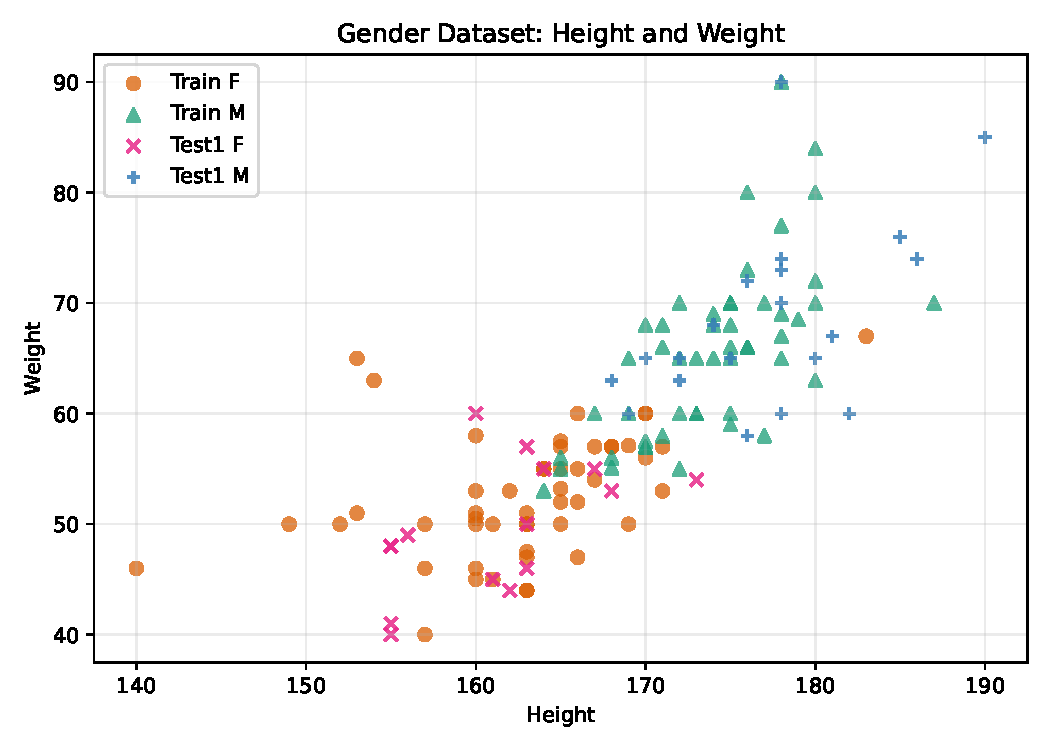
\includegraphics[width=0.72\textwidth]{figures/experiment1/data_scatter.pdf}
\caption{男女训练样本身高--体重散点分布}
\label{fig:exp1_scatter}
\end{figure}

由训练集使用最大似然估计得到的二维高斯参数如下：
\[
\hat{\boldsymbol{\mu}}_F = [162.840,\;52.596]^T,
\quad
\hat{\boldsymbol{\Sigma}}_F=
\begin{bmatrix}
43.934 & 15.525\\
15.525 & 31.129
\end{bmatrix},
\]
\[
\hat{\boldsymbol{\mu}}_M = [173.920,\;65.502]^T,
\quad
\hat{\boldsymbol{\Sigma}}_M=
\begin{bmatrix}
20.754 & 23.058\\
23.058 & 59.898
\end{bmatrix}.
\]
从均值看，男生训练样本的平均身高和平均体重均高于女生；从协方差看，两类样本的身高与体重均呈正相关，说明较高的样本往往也较重。男生协方差中的非对角元素更大，表示男生样本中身高和体重的线性相关更明显。

\subsection{程序框图与代码实现}

\begin{figure}[H]
\centering
\begin{tikzpicture}[node distance=1.2cm, >=stealth, every node/.style={font=\small}]
\tikzstyle{block}=[rectangle, draw, rounded corners, align=center, minimum width=3.2cm, minimum height=0.8cm]
\node[block] (load) {读取训练集与测试集};
\node[block, below=of load] (feature) {选择特征\\身高/体重/二维特征};
\node[block, below=of feature] (estimate) {估计模型参数\\均值、方差、协方差};
\node[block, below=of estimate] (rule) {构造 Bayes 判别函数\\最小错误率/最小风险};
\node[block, below=of rule] (test) {训练集与测试集预测};
\node[block, below=of test] (eval) {计算准确率、召回率、混淆矩阵\\绘制决策边界和密度曲线};
\draw[->] (load) -- (feature);
\draw[->] (feature) -- (estimate);
\draw[->] (estimate) -- (rule);
\draw[->] (rule) -- (test);
\draw[->] (test) -- (eval);
\end{tikzpicture}
\caption{实验一程序流程图}
\label{fig:exp1_flow}
\end{figure}

关键程序位于 \texttt{scripts/experiment1\_bayes.py}。数据读取时先把测试集中的性别标签统一为 \texttt{F} 和 \texttt{M}，避免大小写差异影响评价。
\begin{lstlisting}
def normalize_label(label: str) -> str:
    # 将 Female/Female-like 标签归一化为 F，Male/Male-like 标签归一化为 M
    value = label.strip().upper()
    if value.startswith("F"):
        return "F"
    if value.startswith("M"):
        return "M"
    raise ValueError(f"Unknown label: {label}")


def read_test_file(path: Path) -> Tuple[np.ndarray, np.ndarray]:
    # 测试文件每行包含：身高 体重 性别
    rows = []
    labels = []
    with path.open("r", encoding="utf-8") as f:
        for line in f:
            if not line.strip():
                continue
            height, weight, label = line.split()[:3]
            rows.append((float(height), float(weight)))
            labels.append(normalize_label(label))
    return np.array(rows, dtype=float), np.array(labels)
\end{lstlisting}

参数估计部分直接实现高斯分布的最大似然估计。\texttt{covariance\_mode="full"} 表示考虑身高体重相关，\texttt{covariance\_mode="diag"} 表示假设二者不相关。
\begin{lstlisting}
def fit_gaussian(x, y, features, covariance_mode):
    # 对每一类分别估计均值向量和协方差矩阵
    model = {}
    for label in LABELS:
        class_x = x[y == label][:, features]
        if class_x.ndim == 1:
            class_x = class_x[:, None]
        mean = class_x.mean(axis=0)
        centered = class_x - mean
        cov = centered.T @ centered / len(class_x)  # MLE: 分母为 N
        cov = np.atleast_2d(cov)
        if covariance_mode == "diag":
            cov = np.diag(np.diag(cov))  # 不相关假设：只保留方差
        cov = cov + np.eye(cov.shape[0]) * 1e-6
        model[label] = {"mean": mean, "cov": cov}
    return model
\end{lstlisting}

最小错误率 Bayes 分类器使用对数判别函数，避免直接计算很小的概率密度导致数值下溢。
\begin{lstlisting}
def predict_gaussian(model, x, features, priors):
    # 比较 log p(x|wi) + log P(wi)，得分更大的类别即预测类别
    x_selected = x[:, features]
    if x_selected.ndim == 1:
        x_selected = x_selected[:, None]
    scores = []
    for label, prior in zip(LABELS, priors):
        params = model[label]
        log_px = log_gaussian_density(x_selected, params["mean"], params["cov"])
        scores.append(log_px + math.log(prior))
    score_matrix = np.vstack(scores).T
    return np.array([LABELS[idx] for idx in np.argmax(score_matrix, axis=1)])
\end{lstlisting}

最小风险 Bayes 分类器先由对数后验得分恢复后验概率，再根据损失表计算条件风险。
\begin{lstlisting}
def predict_min_risk(model, x, features, priors,
                     loss_predict_f_when_m=1.0,
                     loss_predict_m_when_f=2.0):
    # 计算两个类别的对数后验得分
    x_selected = x[:, features]
    log_posts = []
    for label, prior in zip(LABELS, priors):
        params = model[label]
        log_posts.append(
            log_gaussian_density(x_selected, params["mean"], params["cov"])
            + math.log(prior)
        )
    log_posts = np.vstack(log_posts).T

    # 对数得分归一化为后验概率
    max_log = np.max(log_posts, axis=1, keepdims=True)
    posts = np.exp(log_posts - max_log)
    posts = posts / posts.sum(axis=1, keepdims=True)

    # 根据损失表计算条件风险，选择风险更小的判决
    posterior_f = posts[:, 0]
    posterior_m = posts[:, 1]
    risk_predict_f = loss_predict_f_when_m * posterior_m
    risk_predict_m = loss_predict_m_when_f * posterior_f
    return np.where(risk_predict_f <= risk_predict_m, "F", "M")
\end{lstlisting}

非参数方法中，Parzen 窗使用高斯核估计类条件密度，$k$ 近邻使用欧氏距离投票。
\begin{lstlisting}
def predict_parzen(train_x, train_y, x, features, priors, bandwidth):
    # 对每个类别估计 Parzen 密度，再代入 Bayes 判别函数
    x_selected = x[:, features]
    class_scores = []
    for label, prior in zip(LABELS, priors):
        samples = train_x[train_y == label][:, features]
        density = parzen_density(x_selected, samples, bandwidth)
        class_scores.append(np.log(density + 1e-300) + math.log(prior))
    scores = np.vstack(class_scores).T
    return np.array([LABELS[idx] for idx in np.argmax(scores, axis=1)])


def predict_knn(train_x, train_y, x, features, k):
    # 找到距离测试样本最近的 k 个训练样本，用多数类别作为预测
    train_selected = train_x[:, features]
    query = x[:, features]
    preds = []
    for row in query:
        distances = np.linalg.norm(train_selected - row, axis=1)
        nearest = np.argsort(distances)[:k]
        labels, counts = np.unique(train_y[nearest], return_counts=True)
        preds.append(sorted(labels[counts == counts.max()])[0])
    return np.array(preds)
\end{lstlisting}

\subsection{实验步骤与结果分析}

\subsubsection{步骤一：单个特征下的最小错误率 Bayes 分类}

首先分别只使用身高和只使用体重作为特征，在一维正态分布假设下估计每类均值和方差，并建立最小错误率 Bayes 分类器。图 \ref{fig:exp1_single_density} 给出了训练样本直方图、估计得到的一维高斯密度曲线以及等先验条件下的分类阈值。

\begin{figure}[H]
\centering
\begin{subfigure}{0.48\textwidth}
\centering
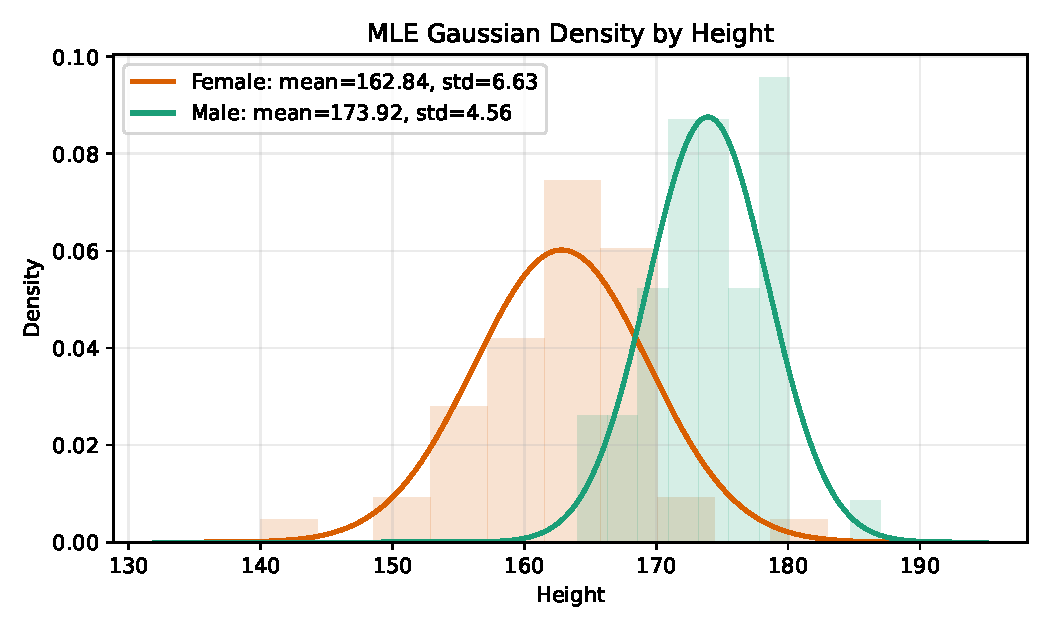
\includegraphics[width=\textwidth]{figures/experiment1/single_feature_height_density.pdf}
\caption{身高特征}
\end{subfigure}
\hfill
\begin{subfigure}{0.48\textwidth}
\centering
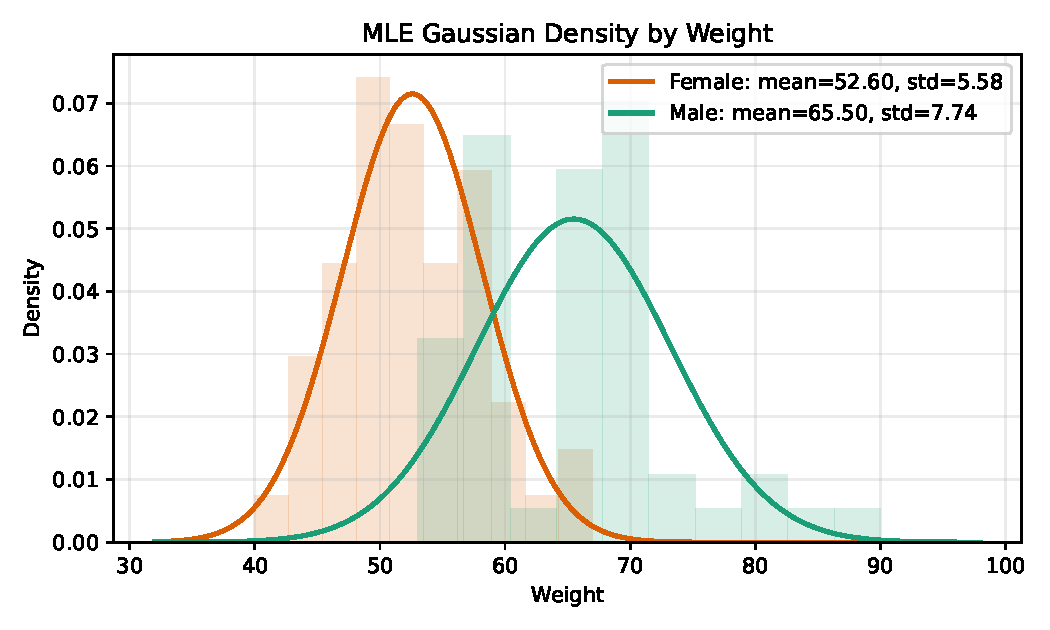
\includegraphics[width=\textwidth]{figures/experiment1/single_feature_weight_density.pdf}
\caption{体重特征}
\end{subfigure}
\caption{单特征高斯密度估计与 Bayes 判决阈值}
\label{fig:exp1_single_density}
\end{figure}

\begin{table}[H]
\centering
\caption{单特征 Bayes 分类准确率（先验概率 $0.5$ vs. $0.5$）}
\begin{tabular}{lccc}
\toprule
特征 & 训练集 & test1 & test2 \\
\midrule
身高 & 86.00\% & 94.29\% & 91.00\% \\
体重 & 82.00\% & 94.29\% & 85.33\% \\
\bottomrule
\end{tabular}
\end{table}

可以看到，身高单特征在训练集和 test2 上均优于体重单特征，说明该数据集中身高对性别区分更稳定。体重也有明显判别能力，但两类体重分布重叠更大，因此在样本较多且类别比例不均衡的 test2 上错误率更高。

\subsubsection{步骤二：两个特征下的 Bayes 分类}

然后同时使用身高和体重两个特征，分别在“相关”和“不相关”假设下建立二维高斯 Bayes 分类器。完整协方差模型对应相关假设，对角协方差模型对应不相关假设。等先验下完整协方差模型的二维决策边界如图 \ref{fig:exp1_bayes_boundary} 所示。

\begin{figure}[H]
\centering
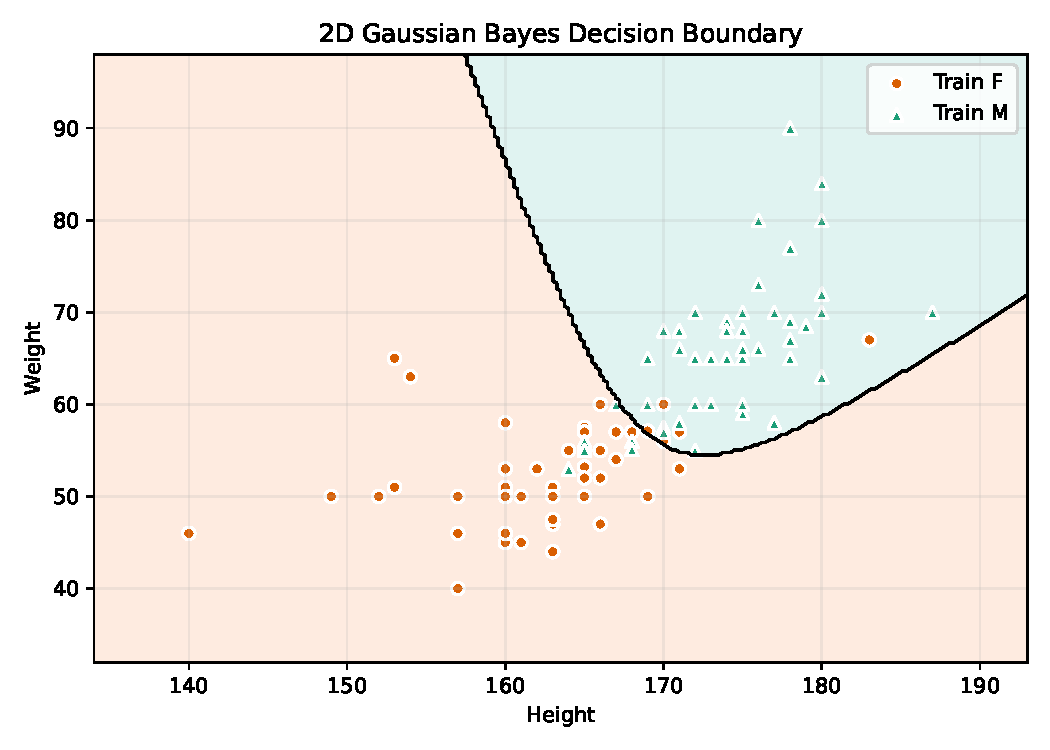
\includegraphics[width=0.75\textwidth]{figures/experiment1/bayes_2d_boundary.pdf}
\caption{二维高斯 Bayes 分类器决策边界}
\label{fig:exp1_bayes_boundary}
\end{figure}

\begin{table}[H]
\centering
\caption{二维特征 Bayes 分类准确率（先验概率 $0.5$ vs. $0.5$）}
\begin{tabular}{lccc}
\toprule
协方差假设 & 训练集 & test1 & test2 \\
\midrule
完整协方差（相关） & 88.00\% & 97.14\% & 89.33\% \\
对角协方差（不相关） & 88.00\% & 97.14\% & 90.33\% \\
\bottomrule
\end{tabular}
\end{table}

二维特征在 test1 上达到 97.14\%，高于单特征实验，说明身高和体重联合使用可以提供更多判别信息。但在 test2 上，对角协方差略优于完整协方差，说明完整协方差虽然表达能力更强，也可能更受训练样本规模和测试集分布差异影响；在样本较少时，较简单的不相关模型反而可能具有更好的泛化表现。

\subsubsection{步骤三：不同先验概率对决策规则的影响}

在 Bayes 判别函数中，先验概率通过 $\ln P(\omega_i)$ 改变决策边界的位置。图 \ref{fig:exp1_prior_boundary} 展示了先验从均衡逐渐偏向女生时，二维 Bayes 决策区域的变化。

\begin{figure}[H]
\centering
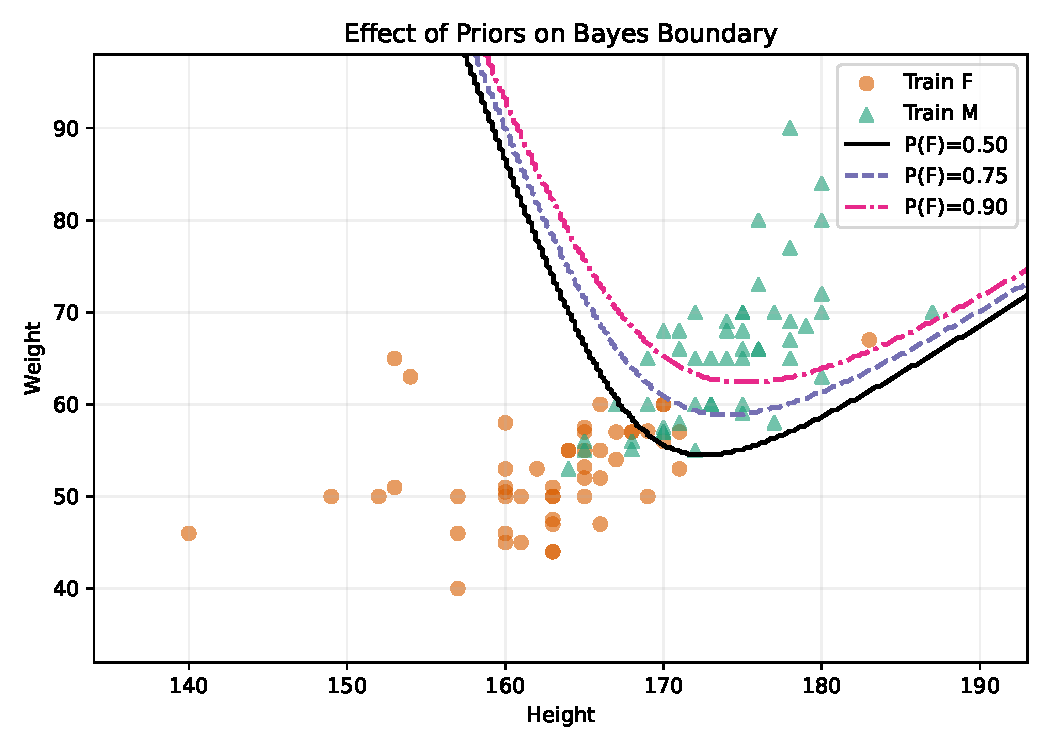
\includegraphics[width=0.82\textwidth]{figures/experiment1/bayes_prior_boundaries.pdf}
\caption{不同先验概率下的 Bayes 决策边界比较}
\label{fig:exp1_prior_boundary}
\end{figure}

\begin{table}[H]
\centering
\caption{不同先验概率下二维完整协方差 Bayes 分类准确率}
\begin{tabular}{lccc}
\toprule
先验概率 $P(F)$ vs. $P(M)$ & 训练集 & test1 & test2 \\
\midrule
0.50 vs. 0.50 & 88.00\% & 97.14\% & 89.33\% \\
0.75 vs. 0.25 & 86.00\% & 85.71\% & 80.00\% \\
0.90 vs. 0.10 & 79.00\% & 80.00\% & 67.33\% \\
\bottomrule
\end{tabular}
\end{table}

由于 test2 中男生占多数，若人为设置更偏向女生的先验，会扩大女生判决区域，使更多男生被误判为女生，因此总体准确率明显下降。这说明先验概率不是随意调节的超参数，而应尽量反映真实应用场景中的类别比例或任务偏好。

\subsubsection{步骤四：最小风险 Bayes 决策}

在表 \ref{tab:exp1_loss} 的损失设定下，女生被错判为男生的损失为 2，男生被错判为女生的损失为 1。因此分类器会更倾向于减少女生漏判。实验结果如下：

\begin{table}[H]
\centering
\caption{最小风险 Bayes 分类准确率}
\begin{tabular}{lccc}
\toprule
方法 & 训练集 & test1 & test2 \\
\midrule
最小风险 Bayes & 84.00\% & 94.29\% & 84.33\% \\
\bottomrule
\end{tabular}
\end{table}

test2 上女生 50 个样本中有 49 个被正确识别，仅 1 个女生被判为男生；但男生中有 46 个被判为女生。也就是说，最小风险决策牺牲了一部分总体准确率，换取了对高损失错误的控制。这体现了模式识别中“最优”与具体任务目标有关：最小错误率追求平均错误少，最小风险追求代价小。

\subsubsection{步骤五：非参数估计实验}

最后实现 Parzen 窗和 $k$ 近邻方法，并与参数化二维 Bayes 分类器比较。图 \ref{fig:exp1_nonparam_boundary} 展示了非参数方法得到的决策边界。

\begin{figure}[H]
\centering
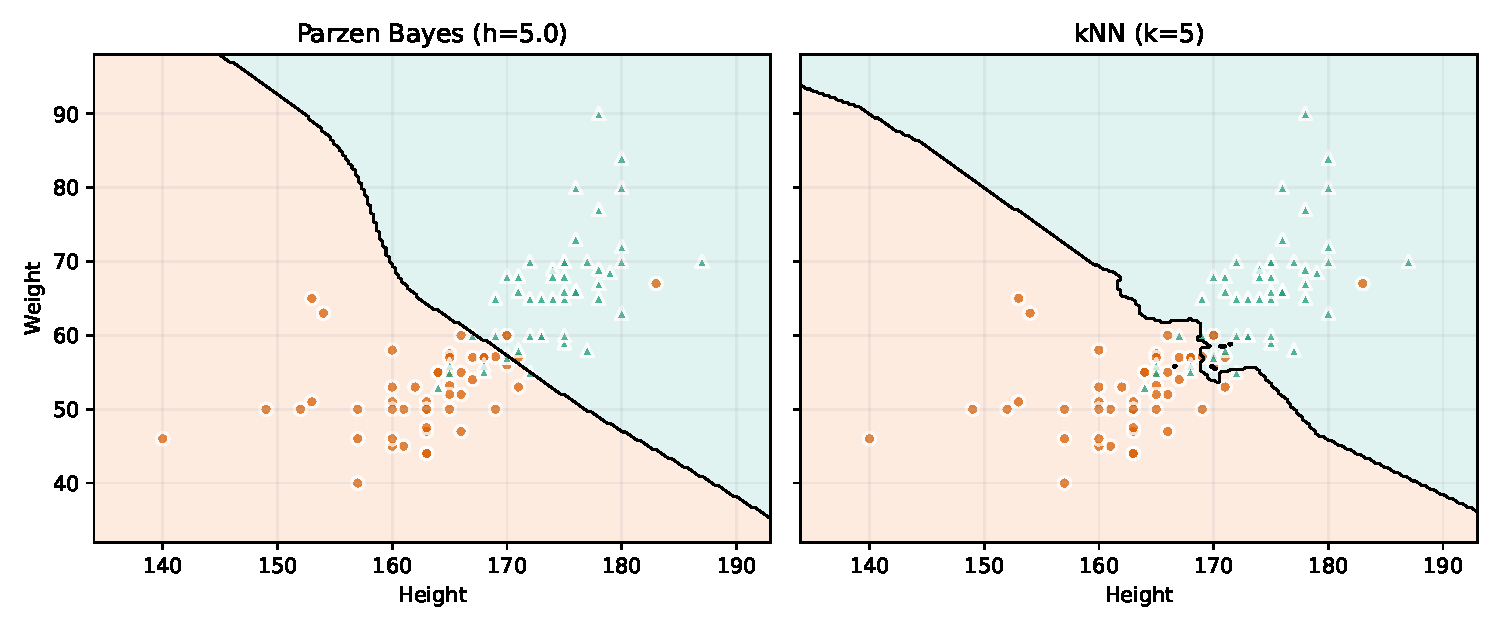
\includegraphics[width=0.82\textwidth]{figures/experiment1/nonparametric_boundaries.pdf}
\caption{Parzen 窗和 $k$ 近邻分类边界}
\label{fig:exp1_nonparam_boundary}
\end{figure}

\begin{table}[H]
\centering
\caption{参数估计与非参数估计分类性能比较}
\begin{tabular}{lccc}
\toprule
方法 & 训练集 & test1 & test2 \\
\midrule
二维高斯 Bayes（完整协方差） & 88.00\% & 97.14\% & 89.33\% \\
Parzen 窗 Bayes & 87.00\% & 97.14\% & 90.33\% \\
$k$ 近邻 & 89.00\% & 100.00\% & 90.33\% \\
\bottomrule
\end{tabular}
\end{table}

Parzen 窗和 $k$ 近邻都不强制数据服从高斯分布，因此边界形状更加灵活。在本数据集中，非参数方法在 test2 上略优于完整协方差高斯 Bayes，但差距不大，说明身高体重数据整体接近可由简单概率模型描述，同时局部非参数方法能对边界附近样本做一定修正。

\subsection{综合实验结果与分析总结}

\begin{table}[H]
\centering
\caption{实验一主要方法汇总结果}
\begin{tabular}{p{3.2cm}p{4.0cm}p{1.8cm}p{1.8cm}p{2.4cm}}
\toprule
方法 & 设置 & 训练准确率 & test1准确率 & test2准确率 \\
\midrule
单特征 Bayes & height; P(F)=0.50, P(M)=0.50 & 86.00\% & 94.29\% & 91.00\% \\
单特征 Bayes & weight; P(F)=0.50, P(M)=0.50 & 82.00\% & 94.29\% & 85.33\% \\
二维相关 Bayes & height\_weight\_full\_cov; P(F)=0.50, P(M)=0.50 & 88.00\% & 97.14\% & 89.33\% \\
二维不相关 Bayes & height\_weight\_diag\_cov; P(F)=0.50, P(M)=0.50 & 88.00\% & 97.14\% & 90.33\% \\
不同先验 Bayes & height\_weight\_full\_cov; P(F)=0.75, P(M)=0.25 & 86.00\% & 85.71\% & 80.00\% \\
不同先验 Bayes & height\_weight\_full\_cov; P(F)=0.90, P(M)=0.10 & 79.00\% & 80.00\% & 67.33\% \\
最小风险 Bayes & height\_weight\_full\_cov; P(F)=0.50, P(M)=0.50; loss M|F=2, loss F|M=1 & 84.00\% & 94.29\% & 84.33\% \\
Parzen Bayes & height\_weight; Gaussian kernel h=5.0; P(F)=0.50, P(M)=0.50 & 87.00\% & 97.14\% & 90.33\% \\
kNN & height\_weight; k=5 & 89.00\% & 100.00\% & 90.33\% \\
\bottomrule
\end{tabular}

\end{table}

\begin{figure}[H]
\centering
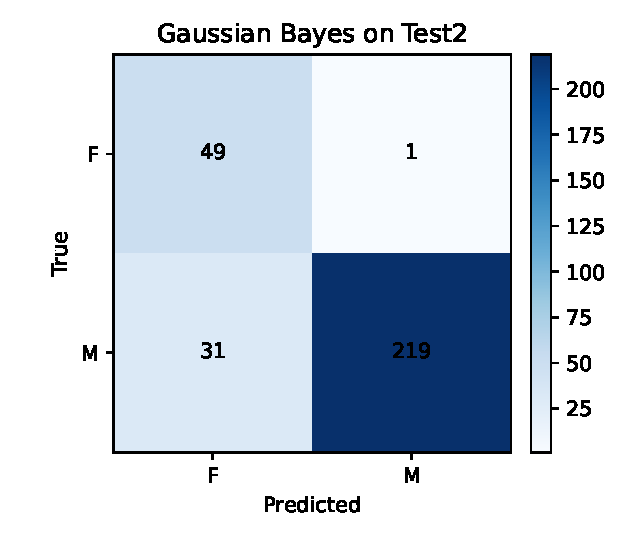
\includegraphics[width=0.55\textwidth]{figures/experiment1/bayes_test2_confusion.pdf}
\caption{二维高斯 Bayes 分类器在 test2 上的混淆矩阵}
\label{fig:exp1_confusion}
\end{figure}

综合来看，本实验可以得到以下结论：
\begin{itemize}
  \item 身高和体重都具有性别判别能力，其中身高单特征更稳定；二维联合特征通常优于单特征。
  \item 完整协方差模型能够描述身高和体重的相关性，但在训练样本较少时，对角协方差模型可能泛化更稳。
  \item 先验概率会直接改变决策边界。若先验与测试集类别比例不一致，可能显著降低总体准确率。
  \item 最小风险 Bayes 决策适合错误代价不对称的任务；它不一定使错误率最低，但能降低指定任务中的期望损失。
  \item 非参数方法减少了分布假设，边界更灵活，但需要选择窗宽或邻居数等超参数，并且对样本规模和局部分布更敏感。
\end{itemize}

\subsection{体会}

通过本实验可以更直观地理解 Bayes 分类器的完整工作链条：先从训练样本估计概率密度，再结合先验概率形成判别函数，最后在测试集上用准确率、召回率和混淆矩阵评价分类器性能。实验也说明，理论公式中的每一项都有实际含义：均值决定类别中心，协方差决定分布形状，先验决定边界偏移，损失函数决定分类器对不同错误的态度。对于模式识别任务，模型并不是越复杂越好，而应结合数据规模、分布假设、类别比例和实际代价共同选择。
\clearpage
\section{实验二：非参数估计、Fisher 线性判别与留一法实验}

\subsection{姓名、学号、班级、题目}

\begin{itemize}
  \item 姓名：\studentname
  \item 学号：\studentid
  \item 班级：\studentclass
  \item 题目：用身高/体重数据进行性别分类的实验（二）
\end{itemize}

\subsection{模式识别理论知识}

实验一主要从概率密度估计出发，在正态分布假设下建立参数化 Bayes 分类器。实验二继续使用男女身高体重数据，重点比较三类思想：非参数概率密度估计、直接设计线性分类器、以及留一法错误率估计。

\subsubsection{非参数估计与 Parzen 窗 Bayes 分类器}

参数估计方法需要先假设概率密度的形式，例如实验一中的二维高斯分布，然后估计均值和协方差。非参数估计则不强行假设类条件概率密度一定服从某种固定分布，而是直接利用训练样本本身估计密度。Parzen 窗就是典型的非参数密度估计方法。

对类别 $\omega_i$，设训练样本为 $\boldsymbol{x}_1,\boldsymbol{x}_2,\ldots,\boldsymbol{x}_{N_i}$，使用高斯核 Parzen 窗估计类条件概率密度：
\[
\hat{p}(\boldsymbol{x}|\omega_i)=
\frac{1}{N_i}\sum_{k=1}^{N_i}
\frac{1}{(2\pi)^{d/2}h^d}
\exp\left[-\frac{1}{2}\left\|\frac{\boldsymbol{x}-\boldsymbol{x}_k}{h}\right\|^2\right].
\]
其中 $d=2$ 表示使用身高和体重两个特征，$h$ 是窗宽。本实验取 $h=5.0$。窗宽越小，密度估计越依赖局部样本，边界更曲折，容易过拟合；窗宽越大，密度估计越平滑，可能忽略真实局部结构。

估计出 $\hat{p}(\boldsymbol{x}|\omega_F)$ 与 $\hat{p}(\boldsymbol{x}|\omega_M)$ 后，仍然使用 Bayes 判别函数：
\[
g_i(\boldsymbol{x})=\ln \hat{p}(\boldsymbol{x}|\omega_i)+\ln P(\omega_i).
\]
若 $g_F(\boldsymbol{x})>g_M(\boldsymbol{x})$，则判为女生，否则判为男生。本实验延续实验一中二维特征、等先验 $P(F)=P(M)=0.5$ 的设置。

\subsubsection{Fisher 线性判别}

Fisher 线性判别是一种直接设计分类器的方法。它不显式估计概率密度，而是寻找一个投影方向 $\boldsymbol{w}$，把二维样本投影到一维轴上，使两类投影后的均值尽量分开，同时每一类内部尽量集中。

设女生和男生的均值向量分别为 $\boldsymbol{\mu}_F$、$\boldsymbol{\mu}_M$，类内散度矩阵为
\[
S_w=\sum_{\boldsymbol{x}\in F}(\boldsymbol{x}-\boldsymbol{\mu}_F)(\boldsymbol{x}-\boldsymbol{\mu}_F)^T+
\sum_{\boldsymbol{x}\in M}(\boldsymbol{x}-\boldsymbol{\mu}_M)(\boldsymbol{x}-\boldsymbol{\mu}_M)^T.
\]
Fisher 准则为
\[
J(\boldsymbol{w})=\frac{\boldsymbol{w}^T S_b\boldsymbol{w}}{\boldsymbol{w}^T S_w\boldsymbol{w}},
\]
最优投影方向可写为
\[
\boldsymbol{w}=S_w^{-1}(\boldsymbol{\mu}_M-\boldsymbol{\mu}_F).
\]
本实验由训练集计算得到
\[
\boldsymbol{w}=[0.002321,\;0.001852]^T,
\quad t=0.500185.
\]
分类时先计算投影值 $y=\boldsymbol{w}^T\boldsymbol{x}$，若 $y\ge t$ 则判为男生，否则判为女生。对应到二维平面中，Fisher 分类器的决策边界是一条直线：
\[
\boldsymbol{w}^T\boldsymbol{x}=t.
\]

\subsubsection{留一法错误率估计}

留一法是一种交叉验证方法。对于 $N$ 个训练样本，每次取出 1 个样本作为验证样本，用剩余 $N-1$ 个样本重新训练分类器，再测试被取出的样本。重复 $N$ 次后，错误率为
\[
\epsilon_{LOO}=\frac{\text{留一过程中错分样本数}}{N}.
\]
留一法的优点是几乎充分利用了训练数据，适合样本数量较少的情况；缺点是计算量较大，因为需要重复训练多次。本实验训练集共有 100 个样本，因此留一法需要对每个分类器重复训练和测试 100 次。

\subsection{实际数据集与实验设置}

本实验仍使用 \texttt{FEMALE.TXT} 和 \texttt{MALE.TXT} 作为训练集，共 100 个样本，其中女生 50 个、男生 50 个；使用 \texttt{test1.txt} 和 \texttt{test2.txt} 作为测试集。特征统一取二维向量
\[
\boldsymbol{x}=[\text{身高},\text{体重}]^T.
\]
实验设置如下：
\begin{itemize}
  \item 参数 Bayes 基线：二维高斯模型，完整协方差矩阵，等先验 $P(F)=P(M)=0.5$。
  \item 非参数 Bayes：高斯核 Parzen 窗，窗宽 $h=5.0$，等先验 $P(F)=P(M)=0.5$。
  \item 线性分类器：Fisher 线性判别，使用训练集计算投影方向和阈值。
  \item 错误率估计：分别计算训练集错误率、test1 错误率、test2 错误率和留一法错误率。
\end{itemize}

\subsection{程序框图与代码实现}

\begin{figure}[H]
\centering
\begin{tikzpicture}[node distance=1.2cm, >=stealth, every node/.style={font=\small}]
\tikzstyle{block}=[rectangle, draw, rounded corners, align=center, minimum width=4.8cm, minimum height=0.8cm]
\node[block] (load) {读取训练集与测试集\\身高、体重、性别};
\node[block, below=of load] (bayes) {建立参数 Bayes 基线\\二维高斯完整协方差};
\node[block, below=of bayes] (parzen) {Parzen 窗估计密度\\得到非参数 Bayes 分类器};
\node[block, below=of parzen] (fisher) {计算 Fisher 投影方向\\得到线性分类边界};
\node[block, below=of fisher] (loo) {留一法重复训练与验证\\估计泛化错误率};
\node[block, below=of loo] (eval) {绘制边界图、投影图、错误率图\\比较实验结果};
\draw[->] (load) -- (bayes);
\draw[->] (bayes) -- (parzen);
\draw[->] (parzen) -- (fisher);
\draw[->] (fisher) -- (loo);
\draw[->] (loo) -- (eval);
\end{tikzpicture}
\caption{实验二程序流程图}
\label{fig:exp2_flow}
\end{figure}

实验二程序位于 \texttt{scripts/experiment2\_linear.py}。Parzen 窗部分先对每一类样本计算核密度，再代入 Bayes 判别函数。
\begin{lstlisting}
def parzen_density(query, samples, bandwidth):
    # query 是待分类样本，samples 是某一类训练样本
    # 使用高斯核函数估计 query 在该类别下的概率密度
    diff = query[:, None, :] - samples[None, :, :]
    exponent = -0.5 * np.sum((diff / bandwidth) ** 2, axis=2)
    coef = 1.0 / ((2 * math.pi) ** (samples.shape[1] / 2)
                  * bandwidth ** samples.shape[1])
    return coef * np.exp(exponent).mean(axis=1)


def predict_parzen(train_x, train_y, query, bandwidth, priors=PRIOR_EQUAL):
    # 分别估计女生和男生的 Parzen 密度，再比较 Bayes 对数得分
    scores = []
    for label, prior in zip(LABELS, priors):
        samples = train_x[train_y == label]
        density = parzen_density(query, samples, bandwidth)
        scores.append(np.log(density + 1e-300) + math.log(prior))
    score_matrix = np.vstack(scores).T
    return np.array([LABELS[idx] for idx in np.argmax(score_matrix, axis=1)])
\end{lstlisting}

Fisher 线性判别部分先计算两类均值和类内散度矩阵，再得到投影方向和阈值。
\begin{lstlisting}
def fit_fisher(x, y):
    # 取出女生和男生样本
    f = x[y == "F"]
    m = x[y == "M"]
    mean_f = f.mean(axis=0)
    mean_m = m.mean(axis=0)

    # 类内散度矩阵 Sw，反映同类样本内部的离散程度
    sw = (f - mean_f).T @ (f - mean_f) + (m - mean_m).T @ (m - mean_m)

    # Fisher 最优投影方向：Sw 的伪逆乘以类均值差
    w = np.linalg.pinv(sw) @ (mean_m - mean_f)

    # 把训练样本投影到一维，并取两类投影均值中点作为阈值
    proj_f = f @ w
    proj_m = m @ w
    threshold = 0.5 * (proj_f.mean() + proj_m.mean())
    direction = 1.0 if proj_m.mean() > proj_f.mean() else -1.0
    return {"w": w, "threshold": np.array([threshold]), "direction": np.array([direction])}


def predict_fisher(model, x):
    # 计算投影值，超过阈值则判为男生，否则判为女生
    scores = x @ model["w"]
    threshold = float(model["threshold"][0])
    direction = float(model["direction"][0])
    is_m = scores >= threshold if direction > 0 else scores < threshold
    return np.where(is_m, "M", "F")
\end{lstlisting}

留一法部分每次屏蔽一个训练样本，用其余样本重新训练模型，再判断被屏蔽样本是否分类正确。
\begin{lstlisting}
def loo_error_fisher(x, y):
    # 对训练集中的每一个样本做一次“留一”验证
    errors = 0
    for idx in range(len(x)):
        mask = np.ones(len(x), dtype=bool)
        mask[idx] = False

        # 用剩余 N-1 个样本重新训练 Fisher 分类器
        model = fit_fisher(x[mask], y[mask])

        # 用训练好的模型预测被留下的这个样本
        pred = predict_fisher(model, x[idx : idx + 1])[0]
        errors += int(pred != y[idx])
    return errors / len(x)
\end{lstlisting}

\subsection{实验步骤与结果分析}

\subsubsection{步骤一：Parzen 窗 Bayes 与参数 Bayes 比较}

首先选择实验一中的二维特征、等先验设置作为基线。参数方法使用二维高斯完整协方差模型，非参数方法使用高斯核 Parzen 窗估计类条件密度。两种方法的决策边界如图 \ref{fig:exp2_parzen_bayes} 所示。

\begin{figure}[H]
\centering
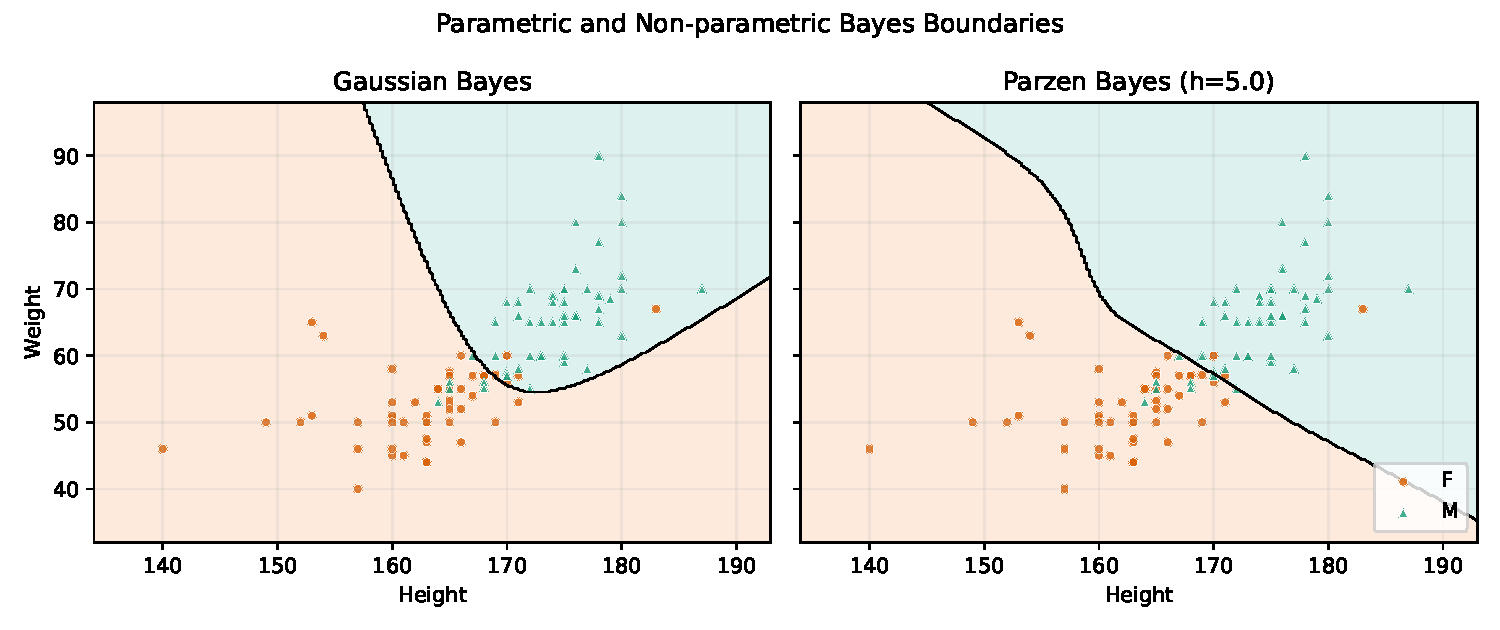
\includegraphics[width=0.90\textwidth]{figures/experiment2/parzen_bayes_boundaries.pdf}
\caption{参数高斯 Bayes 与 Parzen 窗 Bayes 决策边界比较}
\label{fig:exp2_parzen_bayes}
\end{figure}

从图中可以看出，参数高斯 Bayes 的边界主要由两类整体均值和协方差决定，边界形状较规则；Parzen 窗 Bayes 的边界来自训练样本局部核密度叠加，因此更能反映边界附近样本的局部分布。实验中 Parzen 窗 Bayes 的 test2 错误率为 9.67\%，低于参数高斯 Bayes 的 10.67\%，说明非参数密度估计在该数据集上略有提升。

\subsubsection{步骤二：Fisher 线性判别与 Bayes 分类器比较}

接着使用身高和体重两个特征设计 Fisher 线性分类器，并将其与 Bayes 分类器画在同一平面上，如图 \ref{fig:exp2_fisher_bayes} 所示。

\begin{figure}[H]
\centering
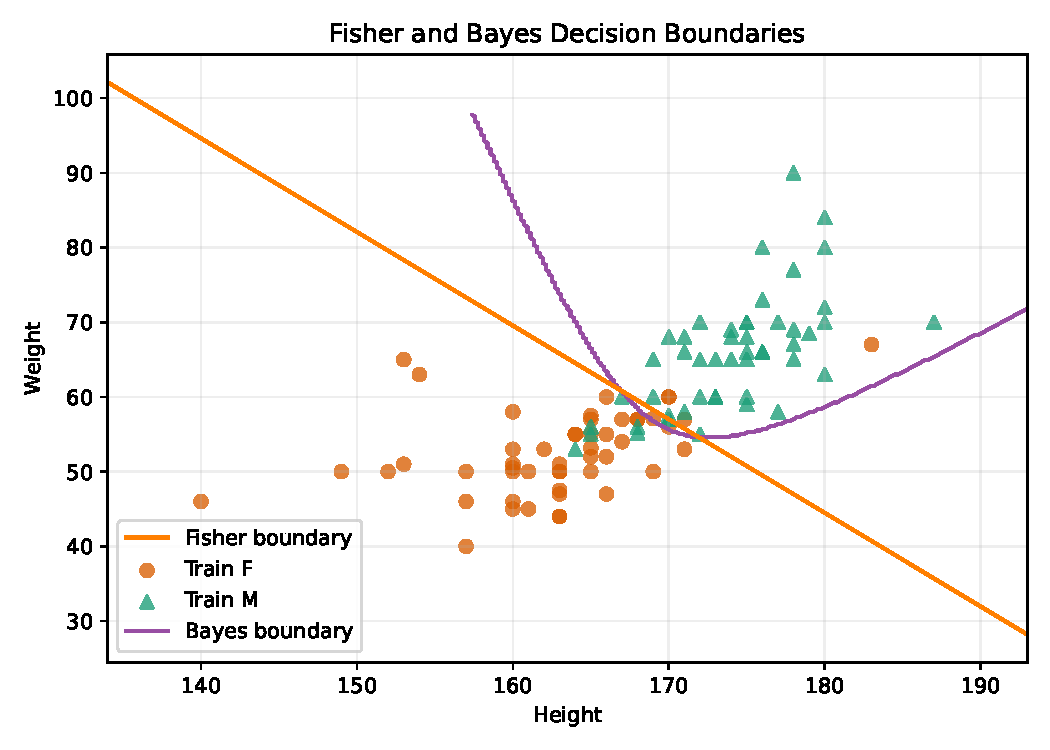
\includegraphics[width=0.76\textwidth]{figures/experiment2/fisher_bayes_boundaries.pdf}
\caption{Fisher 线性判别与 Bayes 分类器决策边界比较}
\label{fig:exp2_fisher_bayes}
\end{figure}

Fisher 分类器得到的是一条直线边界，形式简单，计算量小；Bayes 分类器基于类条件概率密度，边界可以是非线性的。由于男女身高体重数据在二维平面上大体呈左下与右上的分离趋势，线性边界已经能够取得较好效果。Fisher 方法在 test2 上错误率为 9.67\%，与 Parzen 窗 Bayes 相同，略优于参数高斯 Bayes。

训练样本投影到 Fisher 方向后的分布如图 \ref{fig:exp2_projection} 所示。投影后女生样本整体位于较低投影值区域，男生样本整体位于较高投影值区域，中间重叠区域对应分类中最容易出错的样本。

\begin{figure}[H]
\centering
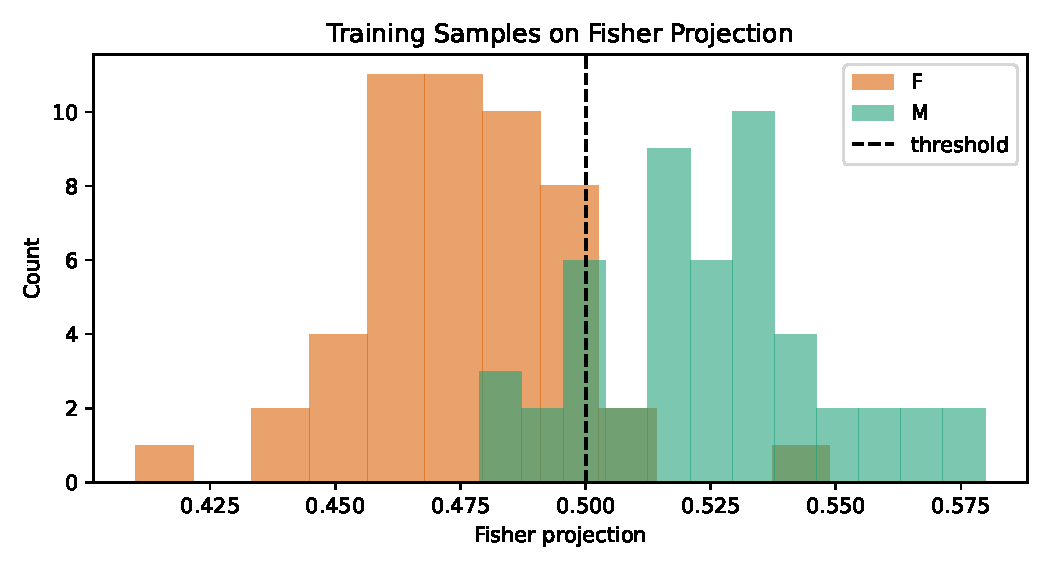
\includegraphics[width=0.76\textwidth]{figures/experiment2/fisher_projection.pdf}
\caption{训练样本在 Fisher 投影方向上的分布}
\label{fig:exp2_projection}
\end{figure}

\subsubsection{步骤三：留一法错误率估计}

最后对参数高斯 Bayes、Parzen 窗 Bayes 和 Fisher 线性判别分别进行留一法估计，并与训练错误率和 test2 错误率比较，如图 \ref{fig:exp2_loo} 和表 \ref{tab:exp2_summary} 所示。

\begin{figure}[H]
\centering
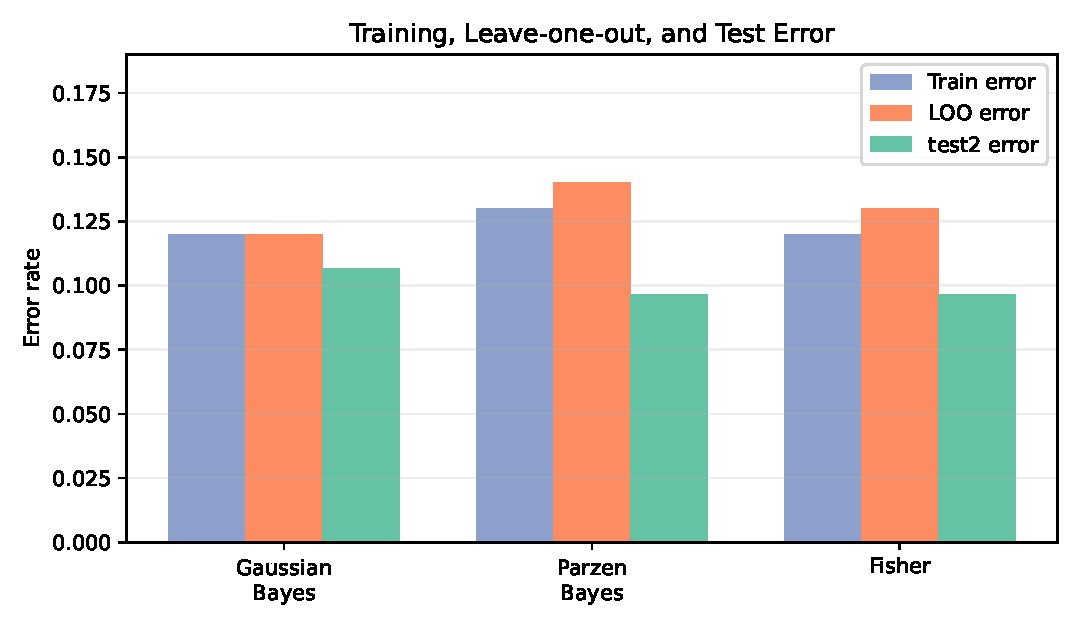
\includegraphics[width=0.74\textwidth]{figures/experiment2/loo_error_comparison.pdf}
\caption{训练错误率、留一法错误率与 test2 错误率比较}
\label{fig:exp2_loo}
\end{figure}

\begin{table}[H]
\centering
\caption{实验二分类器错误率汇总}
\label{tab:exp2_summary}
\small
\begin{tabular}{p{3.0cm}p{2.0cm}p{2.0cm}p{2.0cm}p{2.0cm}}
\toprule
方法 & 训练错误率 & test1错误率 & test2错误率 & 留一法错误率 \\
\midrule
参数高斯 Bayes & 12.00\% & 2.86\% & 10.67\% & 12.00\% \\
Parzen 窗 Bayes & 13.00\% & 2.86\% & 9.67\% & 14.00\% \\
Fisher 线性判别 & 12.00\% & 2.86\% & 9.67\% & 13.00\% \\
\bottomrule
\end{tabular}

\end{table}

留一法结果显示，参数高斯 Bayes、Parzen 窗 Bayes 和 Fisher 线性判别的留一法错误率分别为 12.00\%、14.00\% 和 13.00\%。这些结果与训练错误率和 test2 错误率大体接近，说明留一法能够在训练样本较少时给出较合理的泛化误差估计。test1 错误率均为 2.86\%，明显低于留一法和 test2 错误率，主要原因是 test1 样本量仅 35 个，偶然性更强；test2 样本量为 300 个，更能反映分类器在较大测试集上的表现。

\subsection{综合实验结果与分析总结}

\begin{itemize}
  \item 参数高斯 Bayes 假设类条件概率密度服从二维正态分布，模型结构清晰，训练样本较少时较稳定，但边界形状受分布假设限制。
  \item Parzen 窗 Bayes 不预设固定分布形状，可以利用样本局部结构，test2 错误率由参数 Bayes 的 10.67\% 降至 9.67\%，但对窗宽 $h$ 较敏感。
  \item Fisher 线性判别不估计概率密度，而是直接寻找最佳投影方向；在本数据集上，简单线性边界已能取得与 Parzen 窗 Bayes 相同的 test2 错误率。
  \item 留一法通过重复训练和验证估计泛化误差，适合小样本数据。它比单纯训练错误率更能反映模型面对未知样本时的表现。
\end{itemize}

整体来看，男女身高体重数据具有较明显的线性可分趋势，因此 Fisher 线性判别表现很好；同时，边界附近仍存在局部重叠，Parzen 窗等非参数方法能通过局部密度估计对部分样本做出更灵活的判断。参数 Bayes、非参数 Bayes 和 Fisher 线性判别在本实验中的性能接近，也说明该数据集整体结构比较简单，分类结果更多受边界重叠样本影响。

\subsection{体会}

通过实验二可以体会到，模式识别中分类器设计并不只有“估计概率密度再分类”这一条路线。Bayes 方法强调概率模型，Parzen 窗强调由样本估计局部密度，Fisher 方法则强调直接寻找有判别力的投影方向。三者的出发点不同，但最终都在试图把男女样本有效分开。留一法实验也说明，小样本条件下不能只看训练集表现，应结合交叉验证和独立测试集共同判断模型的泛化能力。
\clearpage
\section{实验三：K-L 变换特征提取实验}

\subsection{姓名、学号、班级、题目}

\begin{itemize}
  \item 姓名：\studentname
  \item 学号：\studentid
  \item 班级：\studentclass
  \item 题目：利用 K-L 变换进行特征提取的实验
\end{itemize}

\subsection{模式识别理论知识}

K-L 变换（Karhunen-Loeve Transform）在模式识别中通常对应主成分分析 PCA。它是一种无监督特征提取方法：不使用样本类别标签，只根据样本整体分布寻找一组正交方向，使样本投影后的方差尽可能集中在前几个方向上。

设原始样本为二维特征向量
\[
\boldsymbol{x}=[\text{身高},\text{体重}]^T,
\]
样本总体均值为 $\boldsymbol{\mu}$，中心化样本为 $\boldsymbol{x}_i-\boldsymbol{\mu}$。总体协方差矩阵为
\[
C=\frac{1}{N}\sum_{i=1}^{N}(\boldsymbol{x}_i-\boldsymbol{\mu})(\boldsymbol{x}_i-\boldsymbol{\mu})^T.
\]
对协方差矩阵做特征值分解：
\[
C\boldsymbol{u}_k=\lambda_k\boldsymbol{u}_k.
\]
其中 $\lambda_k$ 表示沿方向 $\boldsymbol{u}_k$ 的方差大小。最大特征值对应的特征向量 $\boldsymbol{u}_1$ 就是第一主成分方向，即样本整体变化最明显的方向。将样本投影到该方向上可得到一维新特征：
\[
y=\boldsymbol{u}_1^T\boldsymbol{x}.
\]

需要注意的是，K-L/PCA 的目标是“保留总体方差”，不是“最大化类别可分性”。如果类别差异刚好也是总体方差的主要来源，PCA 主方向会有较好的分类能力；如果最大方差来自与类别无关的因素，PCA 方向不一定适合分类。

为了利用类别信息，本实验还使用类平均向量提取判别信息。女生和男生均值分别为 $\boldsymbol{\mu}_F$ 与 $\boldsymbol{\mu}_M$，类均值差方向为
\[
\boldsymbol{w}_{mean}=\frac{\boldsymbol{\mu}_M-\boldsymbol{\mu}_F}{\|\boldsymbol{\mu}_M-\boldsymbol{\mu}_F\|}.
\]
该方向直接指向两类中心分离最大的方向，因此是一种简单的有监督判别投影。分类阈值取两类均值投影的中点：
\[
t=\frac{1}{2}\left(\boldsymbol{w}_{mean}^T\boldsymbol{\mu}_F+\boldsymbol{w}_{mean}^T\boldsymbol{\mu}_M\right).
\]
若 $\boldsymbol{w}_{mean}^T\boldsymbol{x}\ge t$，则判为男生，否则判为女生。

实验二中的 Fisher 线性判别同样利用类别信息，但它不仅考虑两类均值差，还考虑类内散度：
\[
\boldsymbol{w}_{Fisher}=S_w^{-1}(\boldsymbol{\mu}_M-\boldsymbol{\mu}_F).
\]
因此，PCA 主方向、类均值差方向和 Fisher 方向的关系可以概括为：PCA 关注总体方差，类均值差关注类别中心距离，Fisher 同时关注类间分离和类内紧凑。

\subsection{实际数据集与参数计算}

本实验使用 \texttt{FEMALE.TXT} 和 \texttt{MALE.TXT} 中的 100 个训练样本，不使用 \texttt{test1.txt} 和 \texttt{test2.txt} 参与 K-L 方向计算，只用于分类性能测试。将男女训练样本合并后，计算得到总体均值：
\[
\boldsymbol{\mu}=[168.380,\;59.049]^T.
\]
总体协方差矩阵为
\[
C=
\begin{bmatrix}
63.036 & 55.041\\
55.041 & 87.155
\end{bmatrix}.
\]
其特征值为
\[
\lambda_1=131.442,
\quad
\lambda_2=18.748.
\]
对应方差贡献率为
\[
\frac{\lambda_1}{\lambda_1+\lambda_2}=87.52\%,
\quad
\frac{\lambda_2}{\lambda_1+\lambda_2}=12.48\%.
\]
第一主成分方向为
\[
\boldsymbol{u}_1=[0.626888,\;0.779109]^T,
\]
第二主成分方向为
\[
\boldsymbol{u}_2=[-0.779109,\;0.626888]^T.
\]
类均值差方向为
\[
\boldsymbol{w}_{mean}=[0.651392,\;0.758742]^T,
\quad
 t=154.484247.
\]
可以看到，第一主成分方向与类均值差方向非常接近，说明该数据集中总体方差最大的方向基本也是男女类别均值分离的方向。

\subsection{程序框图与代码实现}

\begin{figure}[H]
\centering
\begin{tikzpicture}[node distance=1.2cm, >=stealth, every node/.style={font=\small}]
\tikzstyle{block}=[rectangle, draw, rounded corners, align=center, minimum width=4.8cm, minimum height=0.8cm]
\node[block] (load) {读取男女训练样本\\合并为二维数据矩阵};
\node[block, below=of load] (pca) {中心化并计算协方差矩阵\\特征值分解得到 K-L 主方向};
\node[block, below=of pca] (pcproj) {投影到第一主成分\\设置一维阈值分类};
\node[block, below=of pcproj] (mean) {计算男女类均值差方向\\投影并分类};
\node[block, below=of mean] (compare) {与 Fisher 和 Bayes 比较\\绘制方向、投影和边界图};
\draw[->] (load) -- (pca);
\draw[->] (pca) -- (pcproj);
\draw[->] (pcproj) -- (mean);
\draw[->] (mean) -- (compare);
\end{tikzpicture}
\caption{实验三程序流程图}
\label{fig:exp3_flow}
\end{figure}

实验三程序位于 \texttt{scripts/experiment3\_kl.py}。K-L/PCA 的核心代码如下：
\begin{lstlisting}
def fit_pca_kl(x):
    # 计算总体均值，并对样本中心化
    mean = x.mean(axis=0)
    centered = x - mean

    # 最大似然形式的总体协方差矩阵，分母取样本数 N
    cov = centered.T @ centered / len(x)

    # 对协方差矩阵做特征值分解
    eigvals, eigvecs = np.linalg.eigh(cov)

    # 按特征值从大到小排列，第一列就是第一主成分方向
    order = np.argsort(eigvals)[::-1]
    eigvals = eigvals[order]
    eigvecs = eigvecs[:, order]
    return {"mean": mean, "cov": cov, "eigvals": eigvals, "eigvecs": eigvecs}
\end{lstlisting}

一维投影分类器的实现如下。它既可以用于第一主成分方向，也可以用于类均值差方向。
\begin{lstlisting}
def fit_projection_classifier(x, y, direction):
    # 将二维样本投影到给定方向上，得到一维特征
    proj = x @ direction

    # 分别计算女生和男生在该方向上的投影均值
    mean_f = proj[y == "F"].mean()
    mean_m = proj[y == "M"].mean()

    # 阈值取两个类别投影均值的中点
    threshold = 0.5 * (mean_f + mean_m)
    sign = 1.0 if mean_m > mean_f else -1.0
    return {"direction": direction, "threshold": np.array([threshold]), "sign": np.array([sign])}


def predict_projection(model, x):
    # 根据投影值与阈值的关系进行二分类
    scores = x @ model["direction"]
    threshold = float(model["threshold"][0])
    sign = float(model.get("sign", np.array([1.0]))[0])
    is_m = scores >= threshold if sign > 0 else scores < threshold
    return np.where(is_m, "M", "F")
\end{lstlisting}

类均值差方向直接利用类别标签计算：
\begin{lstlisting}
def fit_mean_direction(x, y):
    # 分别计算男女类别均值
    mean_f = x[y == "F"].mean(axis=0)
    mean_m = x[y == "M"].mean(axis=0)

    # 类均值差方向，并归一化为单位向量
    direction = mean_m - mean_f
    direction = direction / np.linalg.norm(direction)

    # 阈值取两个类均值中点在该方向上的投影
    midpoint = 0.5 * (mean_f + mean_m)
    threshold = float(midpoint @ direction)
    return {"direction": direction, "threshold": np.array([threshold])}
\end{lstlisting}

\subsection{实验步骤与结果分析}

\subsubsection{步骤一：不考虑类别信息的 K-L/PCA 变换}

首先将男女训练样本合并，不使用类别标签，计算总体协方差矩阵及其特征向量。图 \ref{fig:exp3_directions} 中 PC1 表示第一主成分方向，PC2 表示第二主成分方向。可以看到 PC1 沿着身高和体重共同增大的方向，这说明训练样本的主要变化来自“更高更重”和“更矮更轻”的差异。

\begin{figure}[H]
\centering
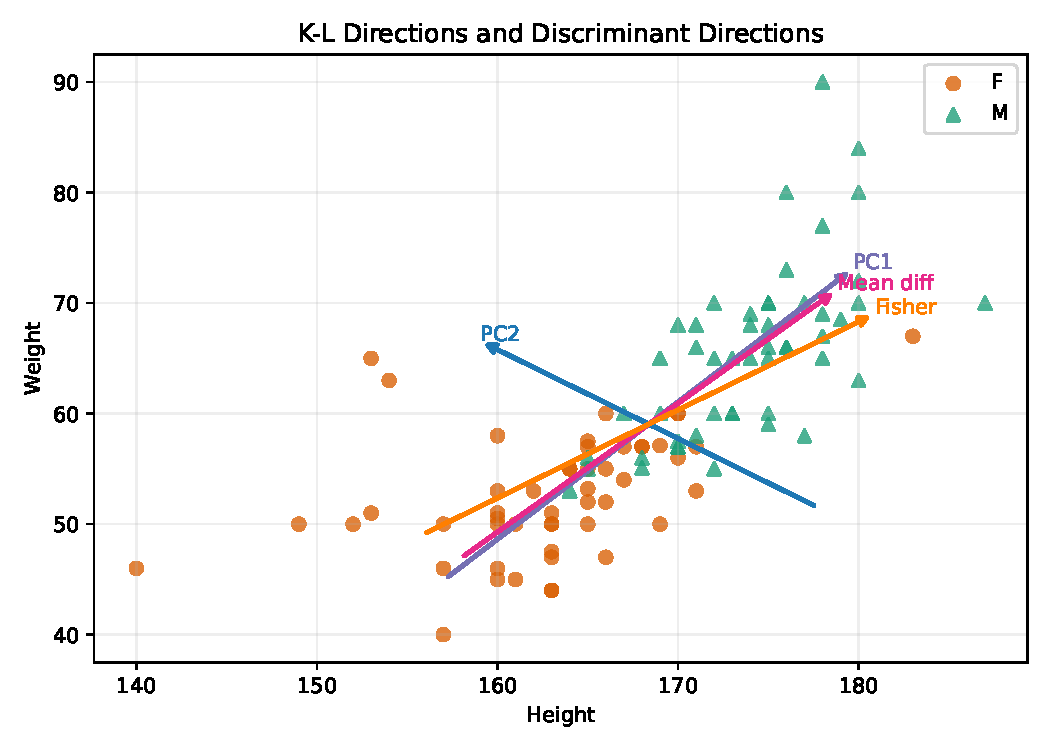
\includegraphics[width=0.74\textwidth]{figures/experiment3/kl_directions.pdf}
\caption{K-L 主方向、类均值差方向与 Fisher 方向比较}
\label{fig:exp3_directions}
\end{figure}

将样本投影到第一主成分方向后，得到图 \ref{fig:exp3_pca_projection}。女生投影值整体偏小，男生投影值整体偏大，中间存在少量重叠，因此可以用一维阈值完成分类。

\begin{figure}[H]
\centering
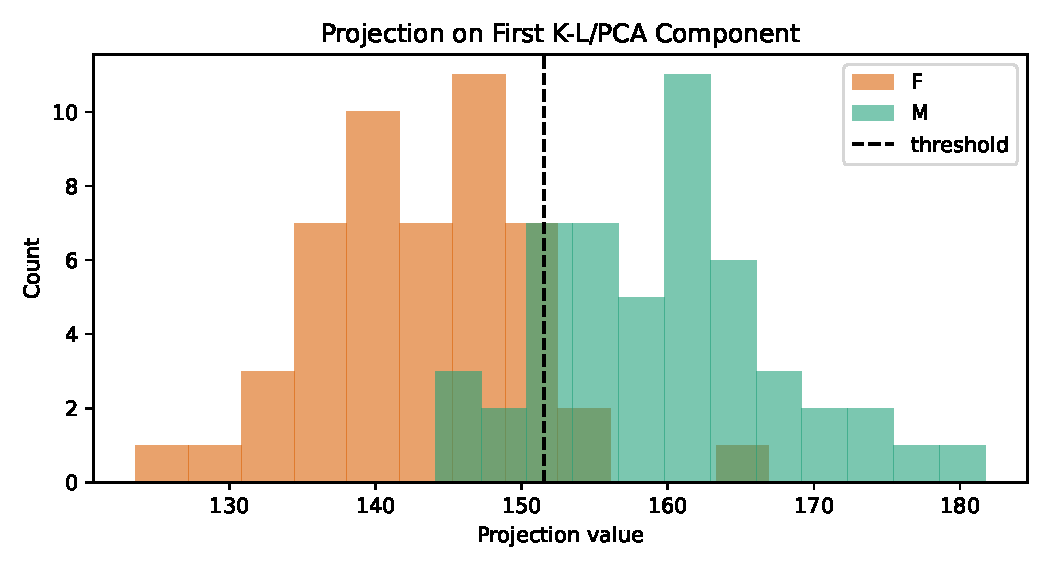
\includegraphics[width=0.74\textwidth]{figures/experiment3/pca_projection.pdf}
\caption{训练样本在 K-L 第一主成分方向上的投影分布}
\label{fig:exp3_pca_projection}
\end{figure}

K-L/PCA 第一主成分分类在训练集上的准确率为 86.00\%，在 \texttt{test1.txt} 上为 100.00\%，在 \texttt{test2.txt} 上为 89.67\%。这说明虽然 PCA 没有使用类别信息，但由于数据主要方差方向与性别差异方向接近，第一主成分仍具有较强判别能力。

\subsubsection{步骤二：利用类平均向量提取判别信息}

第二步利用类别标签，计算男生均值与女生均值的差向量，并将其作为投影方向。该方向直接连接两类中心，因此比 PCA 更具有明确的判别含义。投影结果如图 \ref{fig:exp3_mean_projection} 所示。

\begin{figure}[H]
\centering
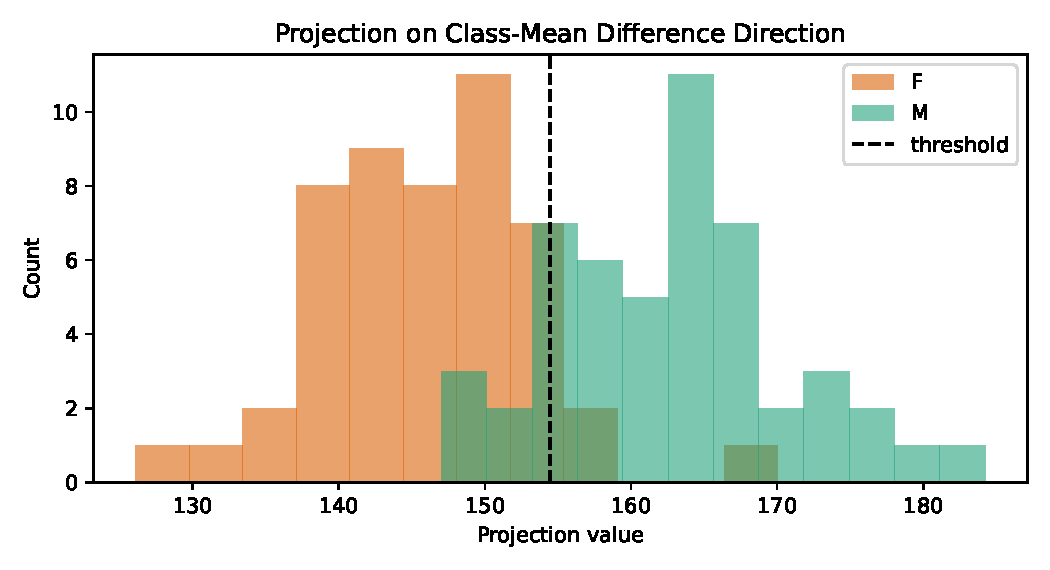
\includegraphics[width=0.74\textwidth]{figures/experiment3/mean_projection.pdf}
\caption{训练样本在类均值差方向上的投影分布}
\label{fig:exp3_mean_projection}
\end{figure}

本实验中，类均值差方向的训练准确率、test1 准确率和 test2 准确率分别为 86.00\%、100.00\% 和 89.67\%，与 K-L/PCA 第一主成分完全相同。这是因为两者方向非常接近，得到的一维投影排序和阈值划分几乎一致。

\subsubsection{步骤三：与 Fisher、Bayes 分类方法比较}

为了比较不同方法的分类面，将 K-L/PCA 主方向、类均值差方向、Fisher 线性判别边界和二维高斯 Bayes 边界画在同一平面上，如图 \ref{fig:exp3_boundaries} 所示。

\begin{figure}[H]
\centering
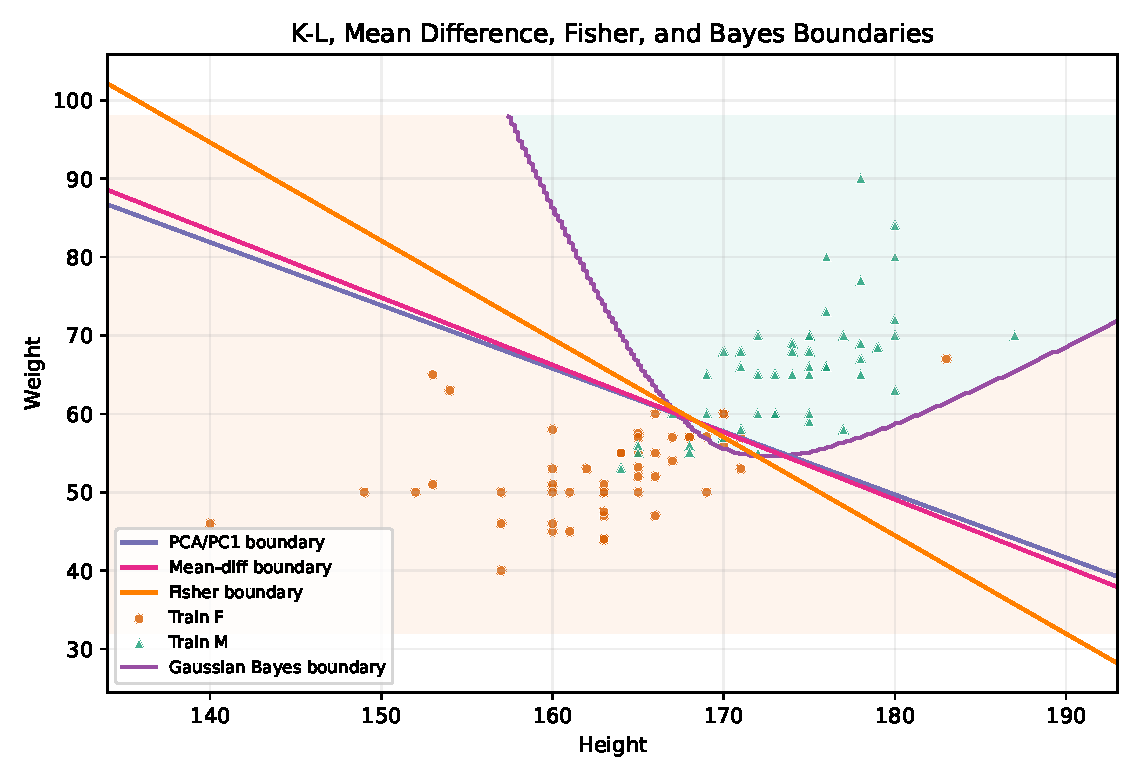
\includegraphics[width=0.78\textwidth]{figures/experiment3/classification_boundaries.pdf}
\caption{K-L、类均值差、Fisher 与 Bayes 分类边界比较}
\label{fig:exp3_boundaries}
\end{figure}

从图中可以看出，K-L/PCA 与类均值差方向对应的线性边界几乎重合，Fisher 边界略有旋转，这是因为 Fisher 还考虑了类内散度；Bayes 边界由概率密度估计得到，可以呈现非线性形状。各方法的准确率对比如表 \ref{tab:exp3_summary} 所示。

\begin{table}[H]
\centering
\caption{实验三 K-L 变换与相关分类方法结果汇总}
\label{tab:exp3_summary}
\small
\begin{tabular}{p{3.0cm}p{2.2cm}p{2.2cm}p{2.2cm}}
\toprule
方法 & 训练准确率 & test1准确率 & test2准确率 \\
\midrule
K-L/PCA 主方向 & 86.00\% & 100.00\% & 89.67\% \\
类均值差方向 & 86.00\% & 100.00\% & 89.67\% \\
Fisher 线性判别 & 88.00\% & 97.14\% & 90.33\% \\
二维高斯 Bayes & 88.00\% & 97.14\% & 89.33\% \\
\bottomrule
\end{tabular}

\end{table}

\subsection{综合实验结果与分析总结}

综合结果可以看出：
\begin{itemize}
  \item K-L/PCA 第一主成分保留了 87.52\% 的总体方差信息，并在 test2 上达到 89.67\% 的准确率，说明它提取到的主要变化方向具有较强性别判别能力。
  \item 类均值差方向与 PCA 第一主成分方向接近，因此分类结果完全相同。这说明本数据集中“总体变化最大方向”和“男女均值分离方向”基本一致。
  \item Fisher 线性判别在 test2 上达到 90.33\%，略高于 PCA 和类均值差方向，因为 Fisher 同时考虑了类间分离和类内散度。
  \item 二维高斯 Bayes 在 test2 上为 89.33\%，与 PCA 方法接近，但它基于概率密度估计，分类边界可以是非线性的。
\end{itemize}

K-L 变换适合作为降维和特征提取工具，但它本身不是专门为分类设计的。对于本实验的身高体重数据，PCA 主方向刚好接近判别方向，因此分类效果较好；在更复杂的数据中，最大方差方向可能来自光照、姿态、尺度等与类别无关的因素，此时仅靠 PCA 主方向分类可能不够理想，需要结合 Fisher、Bayes 或其他监督分类器。

\subsection{体会}

通过本实验可以更清楚地区分无监督特征提取和监督判别分析。K-L/PCA 不使用类别标签，得到的是最能表示数据整体变化的方向；类均值差方向和 Fisher 方法使用类别标签，更关注样本是否容易被分开。本数据集上三种方向非常接近，说明身高和体重的主要变化本身就与性别差异相关。实验也说明，特征提取方法的效果不仅取决于算法，还取决于数据分布是否与分类目标一致。
\clearpage
\section{实验四：基于 K-L 变换的应用实验}

\subsection{姓名、学号、班级、题目}

\begin{itemize}
  \item 姓名：\studentname
  \item 学号：\studentid
  \item 班级：\studentclass
  \item 题目：基于 K-L 变换的图像识别应用实验
\end{itemize}

\subsection{原理简述}

本实验采用课程要求中的“其它数据库”方案，使用仓库已有飞机分类数据集完成基于 K-L 变换的图像识别。
数据集位于 \texttt{experiment/plane\_dataset\_4\_1/}，包含 16 类飞机图像，
训练集 2530 张，测试集 636 张。实验将图像灰度化并缩放为 $32\times 32$，
再展开为 1024 维向量。

图像样本维数较高，直接在原始像素空间中分类容易受到噪声、光照和背景影响。
K-L 变换可以从训练图像中学习一组正交基，将图像投影到低维主成分空间：
\[
  \mathbf{z}=U_k^T(\mathbf{x}-\boldsymbol{\mu}),
\]
其中 $\boldsymbol{\mu}$ 为训练图像均值，$U_k$ 为前 $k$ 个最大特征值对应的特征向量。
在人脸识别中，该方法对应“特征脸”；在本实验中，相同思想用于提取“特征飞机”。

本实验选取 $k=64$ 个主成分作为主要结果。64 维 PCA 特征累计解释方差比例为 89.88\%。
在低维特征空间中，分别使用最近质心分类器和 1 近邻分类器完成飞机类别识别。

\subsection{程序框图}

\begin{figure}[H]
\centering
\begin{tikzpicture}[node distance=1.4cm, >=stealth]
  \tikzstyle{block}=[rectangle, draw, rounded corners, align=center, minimum width=5.2cm, minimum height=0.8cm]
  \node[block] (load) {读取图像训练集和测试集};
  \node[block, below of=load] (pre) {灰度化、缩放、向量化};
  \node[block, below of=pre] (pca) {K-L/PCA 降维};
  \node[block, below of=pca] (clf) {最近邻或传统分类器识别};
  \node[block, below of=clf] (metric) {计算准确率、召回率、混淆矩阵};
  \draw[->] (load) -- (pre);
  \draw[->] (pre) -- (pca);
  \draw[->] (pca) -- (clf);
  \draw[->] (clf) -- (metric);
\end{tikzpicture}
\caption{基于 K-L 变换的图像识别流程}
\end{figure}

\subsection{实验结果及分析总结}

\begin{figure}[H]
\centering
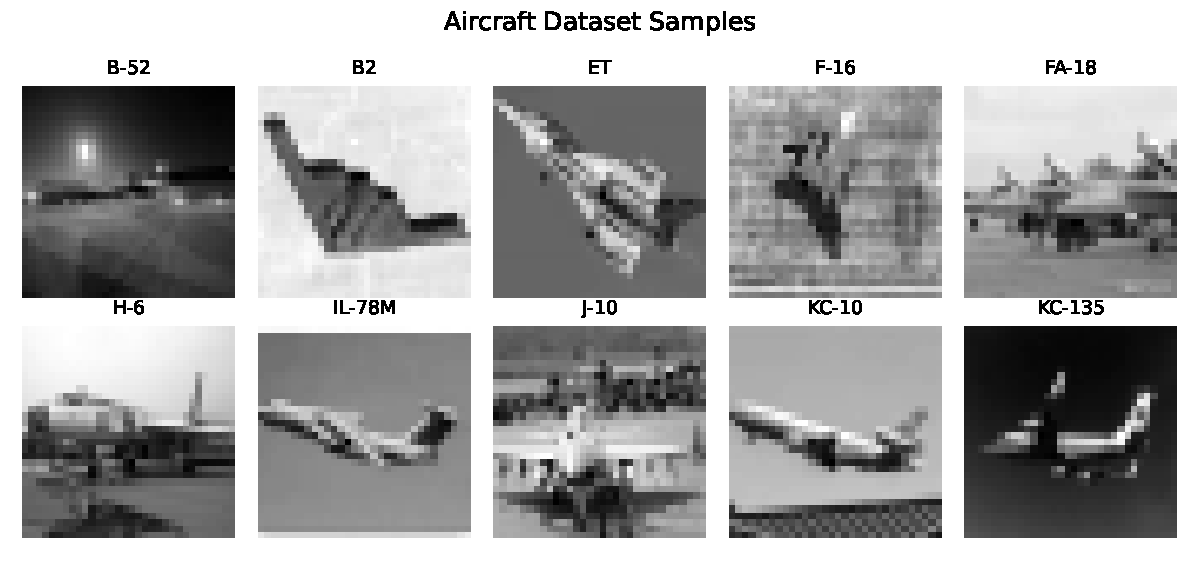
\includegraphics[width=0.76\textwidth]{figures/experiment4/sample_images.pdf}
\caption{飞机分类数据集样本示例}
\end{figure}

\begin{figure}[H]
\centering
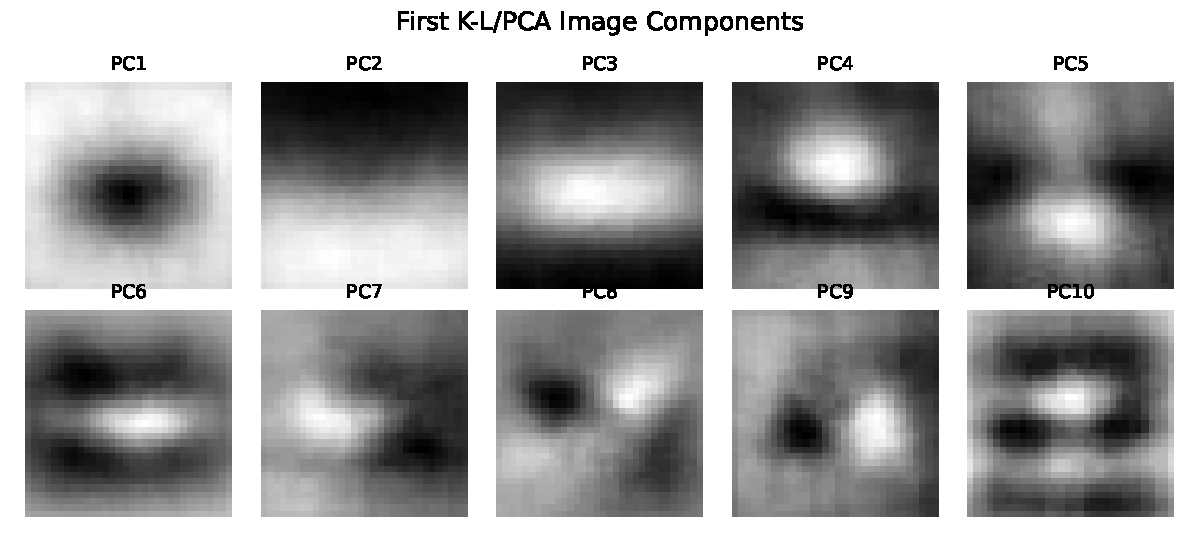
\includegraphics[width=0.76\textwidth]{figures/experiment4/pca_components.pdf}
\caption{K-L/PCA 提取的前 10 个图像主成分}
\end{figure}

\begin{figure}[H]
\centering
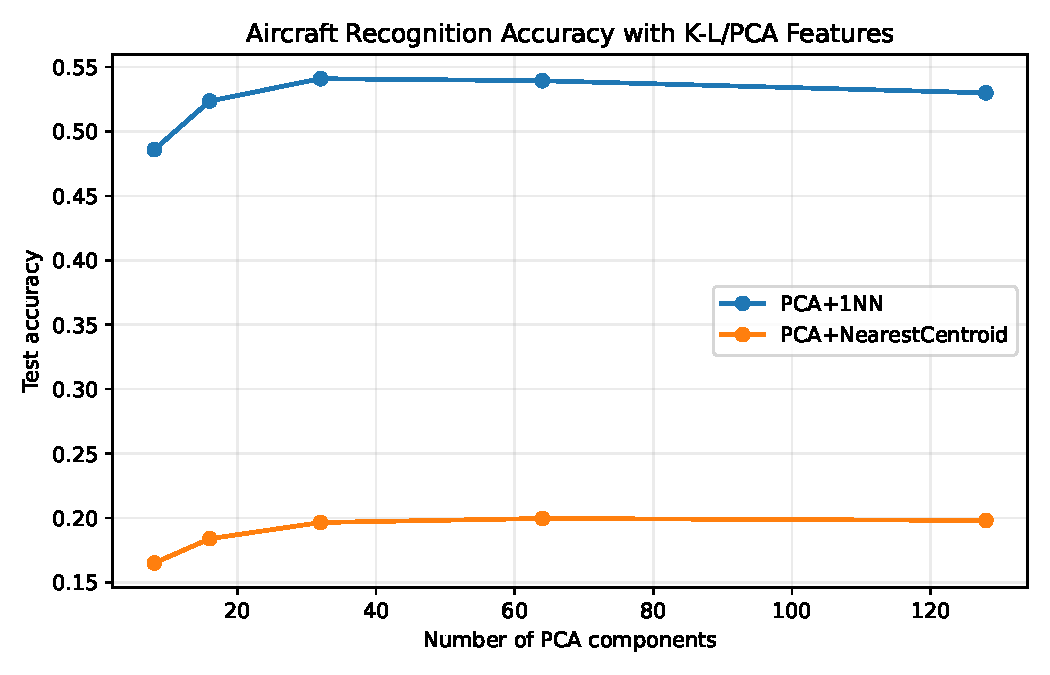
\includegraphics[width=0.72\textwidth]{figures/experiment4/accuracy_vs_components.pdf}
\caption{不同 PCA 主成分数下的测试准确率}
\end{figure}

\begin{table}[H]
\centering
\caption{图像识别实验结果记录表}
\small
\begin{tabular}{p{3.2cm}p{2.2cm}p{2.2cm}p{2.2cm}}
\toprule
方法 & 主成分数 & 训练准确率 & 测试准确率 \\
\midrule
PCA+NearestCentroid & 64 & 20.47\% & 19.97\% \\
PCA+1NN & 64 & 100.00\% & 53.93\% \\
\bottomrule
\end{tabular}

\end{table}

\begin{figure}[H]
\centering
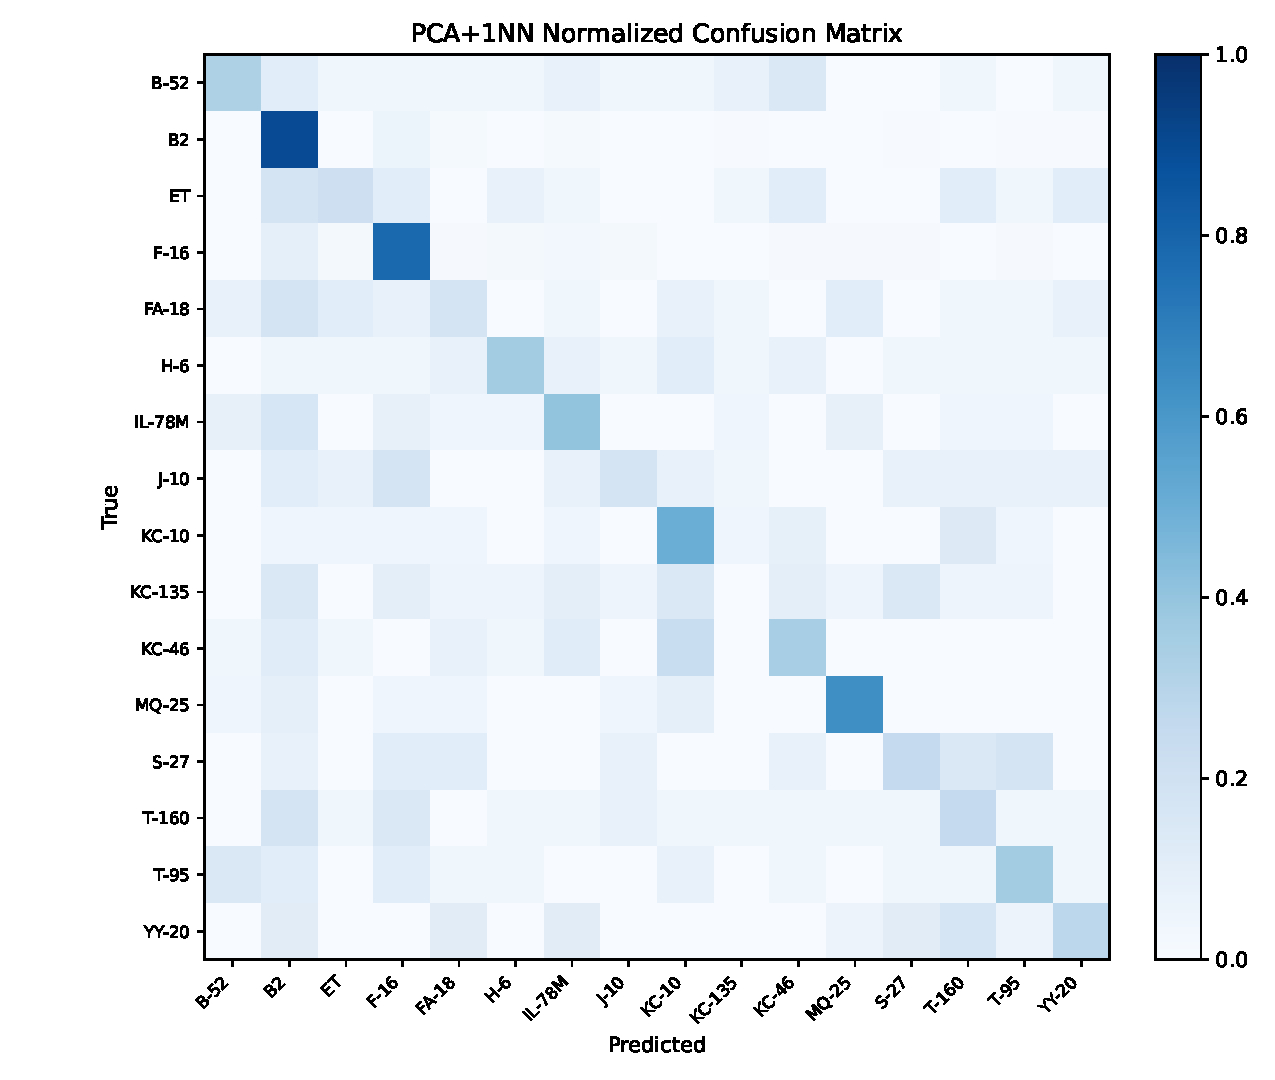
\includegraphics[width=0.78\textwidth]{figures/experiment4/confusion_matrix.pdf}
\caption{PCA+1NN 在飞机测试集上的归一化混淆矩阵}
\end{figure}

从实验结果看，K-L 变换能够有效压缩图像维数。原始灰度图像为 1024 维，
使用 64 个主成分后降至 64 维，同时保留约 89.88\% 的训练集方差信息。
这说明训练图像中存在明显的低维结构，PCA 能够提取主要外形、亮度和纹理变化。

在分类器比较方面，PCA+NearestCentroid 在 64 维下训练准确率为 20.47\%，
测试准确率为 19.97\%。最近质心分类器只用每类均值表示类别，
对同一类别内部姿态、尺度、背景差异较大的飞机图像不够灵活。
PCA+1NN 在训练集上准确率为 100.00\%，测试集准确率为 53.93\%，明显优于最近质心方法。
1NN 能够保留局部样本信息，对飞机图像这类类内变化较大的数据更合适。

从主成分数变化曲线可以看出，PCA+1NN 在 8、16、32、64、128 维下的测试准确率分别约为
48.58\%、52.36\%、54.09\%、53.93\%、52.99\%。主成分数从 8 增加到 32 时准确率提升，
说明更多主成分补充了有效识别信息；但继续增加到 64 或 128 后提升不明显，
甚至略有下降，说明后续主成分可能包含更多背景和噪声。

混淆矩阵显示，不同类别之间仍存在较多混淆。这与飞机图像的姿态、拍摄距离、
背景复杂度和类别不平衡有关。例如部分战斗机或运输机在低分辨率灰度图下外形相似，
仅依靠 PCA 像素特征和简单 1NN 分类器难以完全区分。
因此，K-L 变换适合作为图像识别的基础特征提取方法，
但若要进一步提升准确率，还需要结合更强的图像特征、数据增强或卷积神经网络方法。

\subsection{体会}

通过本实验可以看到，K-L 变换不仅适用于二维身高体重数据，也可以扩展到高维图像识别问题。
图像向量维数很高，而 PCA 可以用较少主成分保留主要变化信息，从而降低计算量并去除部分冗余。
这与“特征脸”方法的思想一致：先从训练图像中学习公共变化方向，再在低维特征空间中完成识别。

同时，本实验也说明，降维并不等于完整解决分类问题。PCA 是无监督方法，
它优先保留总体方差，而这些方差可能来自背景、光照、姿态等与类别无关的因素。
因此 PCA+1NN 能取得一定识别效果，但准确率仍受限。相比之下，最近质心方法过于简单，
无法描述复杂类别分布。后续若要提高飞机图像分类性能，可以考虑监督降维、
方向梯度直方图、SIFT/ORB 特征，或使用卷积神经网络进行端到端特征学习。

\clearpage
\section{实验五：聚类分析实验}

\subsection{姓名、学号、班级、题目}

\begin{itemize}
  \item 姓名：\studentname
  \item 学号：\studentid
  \item 班级：\studentclass
  \item 题目：对数据进行聚类分析的实验
\end{itemize}

\subsection{模式识别理论知识}

前面几个实验主要是监督分类：训练样本带有性别标签，分类器利用标签学习判别规则。聚类分析属于无监督学习，算法只看到样本的特征向量，不使用真实性别标签。聚类的目标是根据样本之间的相似性自动形成若干组，再观察这些组是否与真实类别具有对应关系。

本实验使用二维特征
\[
\boldsymbol{x}=[\text{身高},\text{体重}]^T.
\]
由于身高和体重的量纲及数值范围不同，聚类前先进行标准化：
\[
z_{ij}=\frac{x_{ij}-\mu_j}{\sigma_j}.
\]
这样可以避免某个数值尺度较大的特征在欧氏距离中占据过大影响。

\subsubsection{C 均值聚类}

C 均值聚类也常称为 $k$-means 聚类。给定聚类数 $C$，算法希望找到 $C$ 个聚类中心，使样本到所属中心的平方距离总和最小。目标函数为
\[
J=\sum_{j=1}^{C}\sum_{\boldsymbol{x}_i\in \omega_j}\|\boldsymbol{x}_i-\boldsymbol{\mu}_j\|^2.
\]
其中 $\omega_j$ 表示第 $j$ 个簇，$\boldsymbol{\mu}_j$ 表示该簇中心。算法迭代执行两步：
\[
\omega_i=\arg\min_j\|\boldsymbol{x}_i-\boldsymbol{\mu}_j\|^2,
\]
\[
\boldsymbol{\mu}_j=\frac{1}{N_j}\sum_{\boldsymbol{x}_i\in \omega_j}\boldsymbol{x}_i.
\]
第一步把样本分配给最近中心，第二步用簇内样本均值更新中心，直到中心变化很小或达到最大迭代次数。

C 均值的优点是简单、快速、易实现；缺点是需要预先指定类别数 $C$，对初始中心和特征尺度敏感，并且倾向于发现近似球形的簇。

\subsubsection{聚类指标}

为了分析聚类效果，本实验使用以下指标：
\begin{itemize}
  \item SSE：类内平方误差和，即 C 均值目标函数。SSE 越小表示簇内越紧凑，但它会随着聚类数增加而自然下降。
  \item 轮廓系数：综合衡量簇内紧凑性和簇间分离性，取值越大通常说明聚类结构越清晰。
  \item ARI：调整兰德指数，用真实标签与聚类结果比较。ARI 越大表示聚类结果越接近真实类别。
  \item 性别匹配率：由于聚类编号本身没有性别含义，将两个簇与男女标签做最佳匹配后计算准确率，仅用于解释聚类结果与性别标签的对应程度。
\end{itemize}

\subsubsection{分级聚类}

分级聚类通过逐步合并或分裂样本形成层次结构。本实验采用凝聚式 Ward 分级聚类：初始时每个样本单独成簇，然后不断合并使类内平方误差增加最小的两个簇。Ward 方法不需要随机初始中心，可以用树状图观察样本逐层合并的过程，但当样本数量较大时计算量较高。

\subsection{实际数据集与实验设置}

实验五使用两组数据：
\begin{itemize}
  \item 训练集：\texttt{FEMALE.TXT} 与 \texttt{MALE.TXT} 合并，共 100 个样本，其中女生 50 个、男生 50 个。
  \item 合并数据：训练集再加入 \texttt{test2.txt}，共 400 个样本。由于 \texttt{test2.txt} 中有 50 个女生、250 个男生，因此合并后类别比例变为女生 100 个、男生 300 个。
\end{itemize}

实验步骤如下：
\begin{itemize}
  \item 对训练集设 $C=2$，独立实现 C 均值聚类，并考察不同初始值的影响。
  \item 对训练集分别设置 $C=2,3,4,5$，画出 SSE 和轮廓系数随类别数变化的曲线。
  \item 对训练集使用 Ward 分级聚类，绘制树状图和二维聚类结果。
  \item 将训练集与 \texttt{test2.txt} 合并，重复 C 均值和 Ward 聚类实验，观察样本规模和类别比例变化带来的影响。
\end{itemize}

\subsection{程序框图与代码实现}

\begin{figure}[H]
\centering
\begin{tikzpicture}[node distance=1.2cm, >=stealth, every node/.style={font=\small}]
\tikzstyle{block}=[rectangle, draw, rounded corners, align=center, minimum width=5.2cm, minimum height=0.8cm]
\node[block] (load) {读取训练集或训练集+test2\\身高、体重、性别标签仅用于评价};
\node[block, below=of load] (scale) {标准化身高和体重\\统一距离尺度};
\node[block, below=of scale] (cmeans) {独立实现 C 均值聚类\\样本分配与中心更新};
\node[block, below=of cmeans] (kselect) {改变类别数和初始中心\\计算 SSE、轮廓系数、ARI};
\node[block, below=of kselect] (hier) {Ward 分级聚类\\绘制树状图和二维聚类图};
\node[block, below=of hier] (compare) {比较训练集与合并数据\\分析聚类结构变化};
\draw[->] (load) -- (scale);
\draw[->] (scale) -- (cmeans);
\draw[->] (cmeans) -- (kselect);
\draw[->] (kselect) -- (hier);
\draw[->] (hier) -- (compare);
\end{tikzpicture}
\caption{实验五聚类分析流程图}
\label{fig:exp5_flow}
\end{figure}

实验五程序位于 \texttt{scripts/experiment5\_clustering.py}。C 均值部分为独立编程实现，核心代码如下：
\begin{lstlisting}
def c_means(x, n_clusters, seed, max_iter=200, tol=1e-6):
    # 随机选择 C 个样本作为初始聚类中心
    rng = np.random.default_rng(seed)
    indices = rng.choice(len(x), size=n_clusters, replace=False)
    centers = x[indices].copy()
    labels = np.zeros(len(x), dtype=int)

    for iteration in range(1, max_iter + 1):
        # 计算每个样本到每个中心的欧氏距离
        distances = np.linalg.norm(x[:, None, :] - centers[None, :, :], axis=2)

        # 将样本分配给距离最近的中心
        new_labels = distances.argmin(axis=1)
        new_centers = centers.copy()

        # 根据当前簇内样本均值更新中心
        for cluster in range(n_clusters):
            members = x[new_labels == cluster]
            if len(members) == 0:
                new_centers[cluster] = x[rng.integers(0, len(x))]
            else:
                new_centers[cluster] = members.mean(axis=0)

        # 若中心移动量很小，则认为算法收敛
        shift = np.linalg.norm(new_centers - centers)
        centers = new_centers
        labels = new_labels
        if shift < tol:
            break

    # SSE：样本到所属中心的平方距离总和
    inertia = float(np.sum((x - centers[labels]) ** 2))
    return labels, centers, inertia, iteration
\end{lstlisting}

聚类指标计算与不同类别数实验如下：
\begin{lstlisting}
def evaluate_k_range(x_scaled, y, dataset_name):
    # 分别测试 C=2,3,4,5，记录 SSE、轮廓系数和 ARI
    rows = []
    for n_clusters in range(2, 6):
        labels, centers, inertia, iterations = c_means(
            x_scaled, n_clusters, seed=2026 + n_clusters
        )
        rows.append({
            "dataset": dataset_name,
            "method": "C-means",
            "n_clusters": n_clusters,
            "inertia": inertia,
            "silhouette": silhouette_score(x_scaled, labels),
            "ari": adjusted_rand_score(y, labels),
            "iterations": iterations,
        })
    return rows
\end{lstlisting}

Ward 分级聚类使用已有程序完成，代码如下：
\begin{lstlisting}
def evaluate_hierarchical(x_scaled, y, dataset_name):
    # Ward 分级聚类：每次合并使类内平方误差增加最小的簇
    clustering = AgglomerativeClustering(n_clusters=2, linkage="ward")
    labels = clustering.fit_predict(x_scaled)
    return {
        "dataset": dataset_name,
        "method": "Hierarchical Ward",
        "n_clusters": 2,
        "silhouette": silhouette_score(x_scaled, labels),
        "ari": adjusted_rand_score(y, labels),
        "gender_accuracy_if_2": best_label_accuracy(y, labels),
    }
\end{lstlisting}

\subsection{实验步骤与结果分析}

\subsubsection{步骤一：训练集上 C=2 的 C 均值聚类与初始值影响}

首先将 \texttt{FEMALE.TXT} 和 \texttt{MALE.TXT} 合并，使用身高和体重两个特征，设 $C=2$ 进行 C 均值聚类。结果如图 \ref{fig:exp5_cmeans_train} 所示。

\begin{figure}[H]
\centering
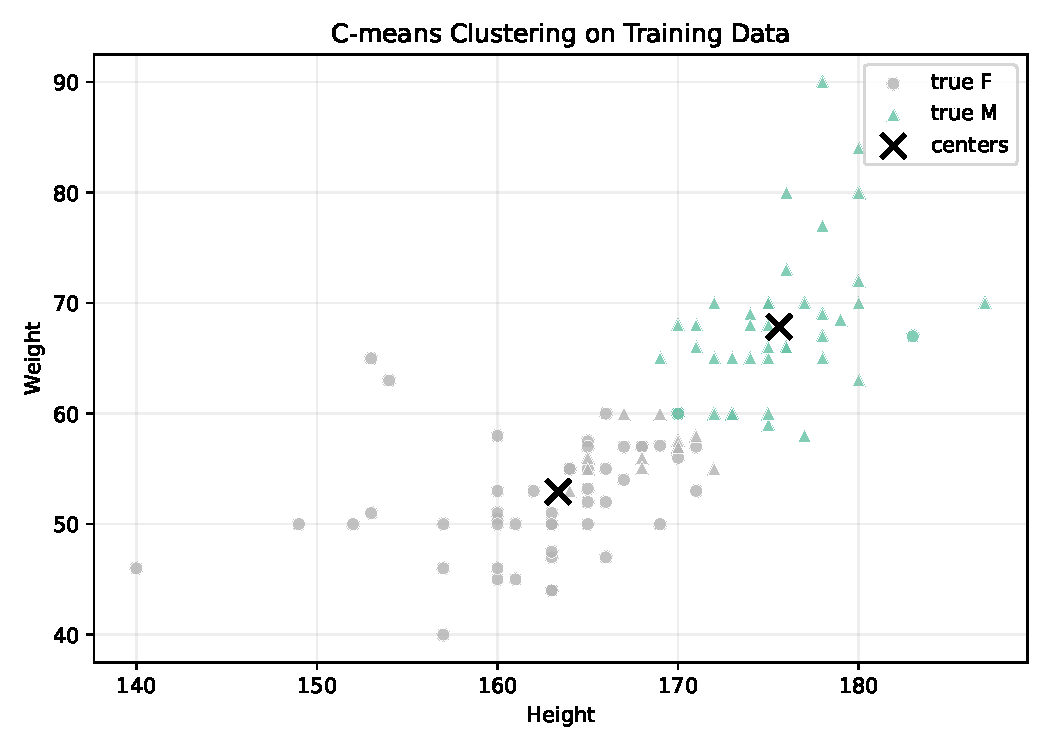
\includegraphics[width=0.74\textwidth]{figures/experiment5/cmeans_train_2clusters.pdf}
\caption{训练集 C 均值聚类结果，$C=2$}
\label{fig:exp5_cmeans_train}
\end{figure}

聚类结果大致形成“较矮较轻”和“较高较重”两个簇，与男女样本的统计差异基本一致。虽然聚类算法没有使用性别标签，但最佳性别匹配率达到 85.00\%，说明身高体重特征中确实存在明显的自然分组结构。

为考察初始中心影响，对 $C=2$ 使用 10 个不同随机种子重复实验，结果如图 \ref{fig:exp5_init} 所示。

\begin{figure}[H]
\centering
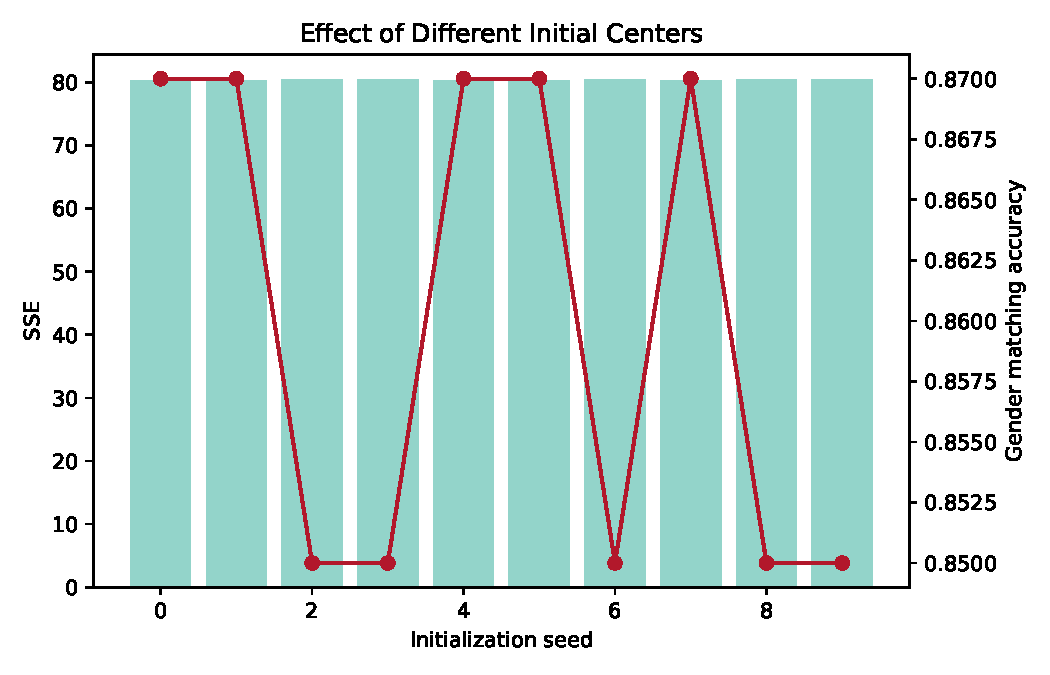
\includegraphics[width=0.74\textwidth]{figures/experiment5/init_variation.pdf}
\caption{不同初始中心对 C 均值聚类结果的影响}
\label{fig:exp5_init}
\end{figure}

不同初始值下 SSE 在 80.3193 到 80.3950 之间变化，性别匹配率在 85.00\% 到 87.00\% 之间变化。说明该数据集聚类结构较稳定，但边界附近样本仍可能因初始中心不同而改变归属。因此实际使用 C 均值时，应多次初始化并选择 SSE 较小的结果。

\subsubsection{步骤二：不同类别数下的聚类指标}

在训练集上分别设置 $C=2,3,4,5$，记录 SSE 和轮廓系数，如图 \ref{fig:exp5_k_train} 所示。

\begin{figure}[H]
\centering
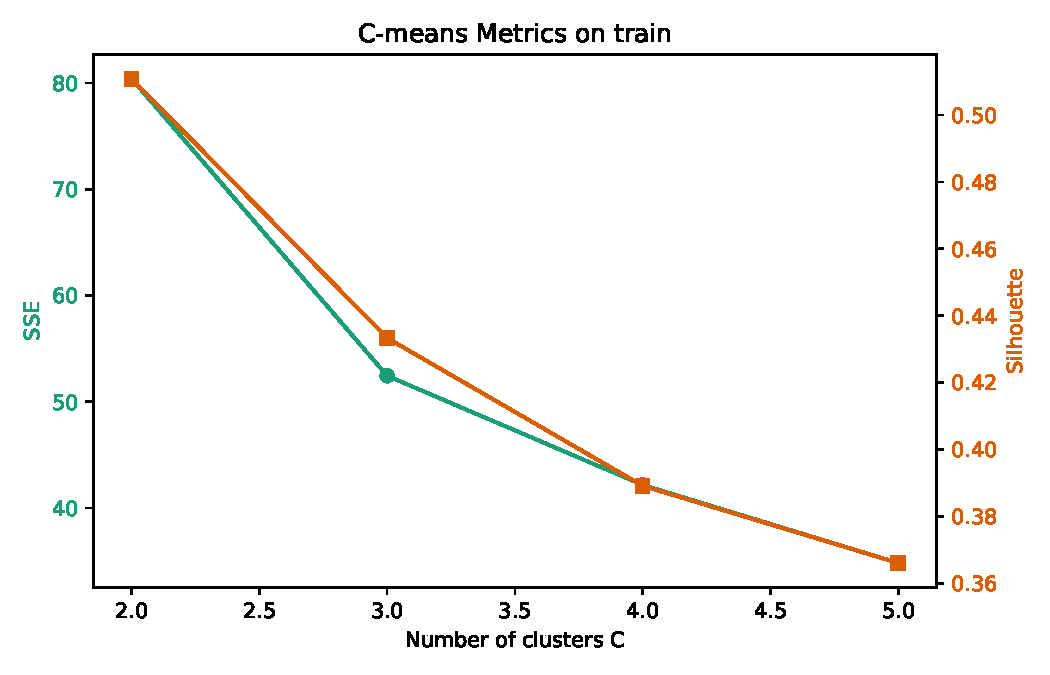
\includegraphics[width=0.74\textwidth]{figures/experiment5/cmeans_k_metrics_train.pdf}
\caption{训练集上不同类别数的 C 均值聚类指标}
\label{fig:exp5_k_train}
\end{figure}

训练集上 $C=2,3,4,5$ 的 SSE 分别为 80.3950、52.4481、42.1838、34.8358。SSE 随类别数增加单调下降，这是因为更多中心必然能降低类内平方误差。但轮廓系数分别为 0.5108、0.4333、0.3891、0.3660，随类别数增加下降。综合来看，$C=2$ 的轮廓系数最高，且与男女两类的先验认知一致，因此训练集上合理类别数更倾向于 2。

\subsubsection{步骤三：Ward 分级聚类}

对训练集使用 Ward 分级聚类，树状图如图 \ref{fig:exp5_dendrogram} 所示，取两类后的二维聚类结果如图 \ref{fig:exp5_hier_train} 所示。

\begin{figure}[H]
\centering
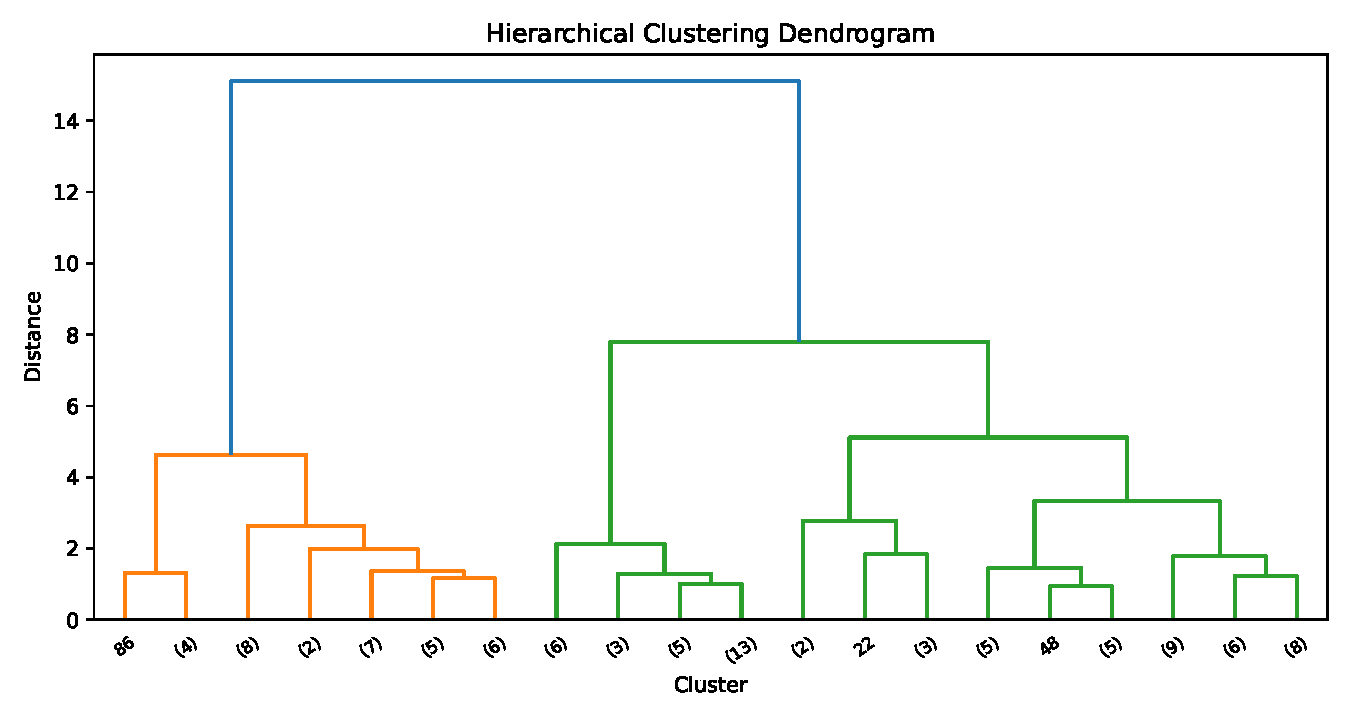
\includegraphics[width=0.82\textwidth]{figures/experiment5/hierarchical_dendrogram_train.pdf}
\caption{训练集 Ward 分级聚类树状图}
\label{fig:exp5_dendrogram}
\end{figure}

\begin{figure}[H]
\centering
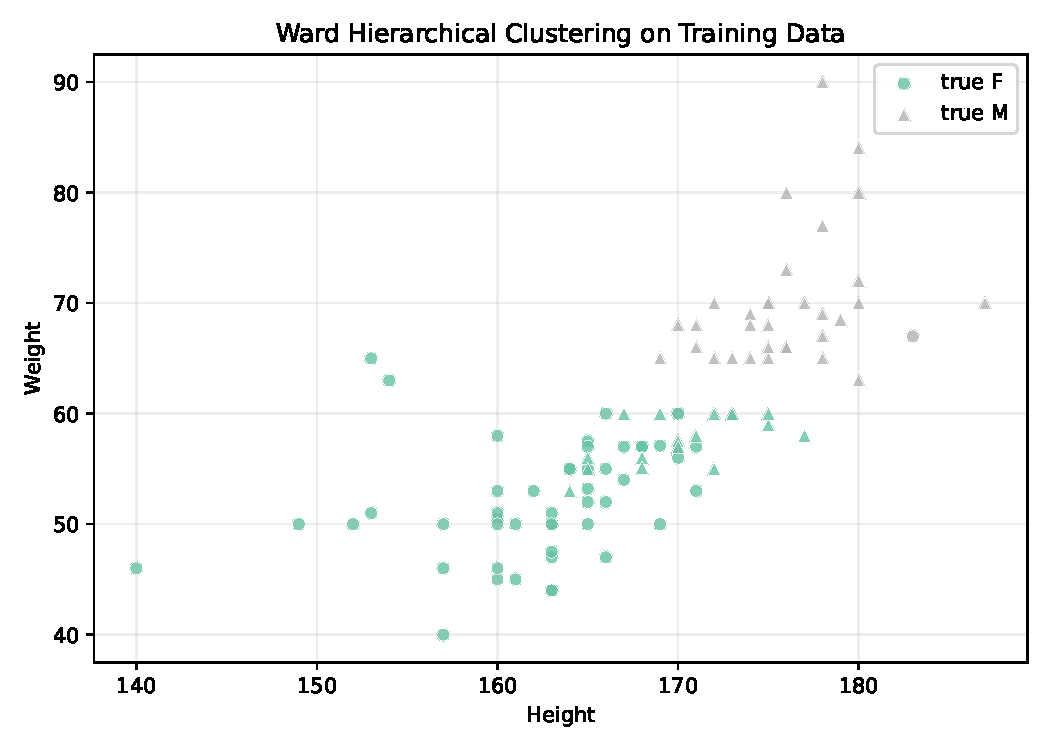
\includegraphics[width=0.74\textwidth]{figures/experiment5/hierarchical_train_2clusters.pdf}
\caption{训练集 Ward 分级聚类结果，$C=2$}
\label{fig:exp5_hier_train}
\end{figure}

Ward 分级聚类在训练集上取两类时，轮廓系数为 0.5049，ARI 为 0.3789，性别匹配率为 81.00\%。其性别匹配率略低于 C 均值，但分级聚类的优势在于可以通过树状图观察样本逐层合并的过程，不依赖随机初始中心。

\subsubsection{步骤四：加入 test2 后重复实验}

最后将训练集与 \texttt{test2.txt} 合并，共 400 个样本，其中男生比例明显升高。对合并数据重复 $C=2$ 的 C 均值聚类，结果如图 \ref{fig:exp5_cmeans_combined} 所示。

\begin{figure}[H]
\centering
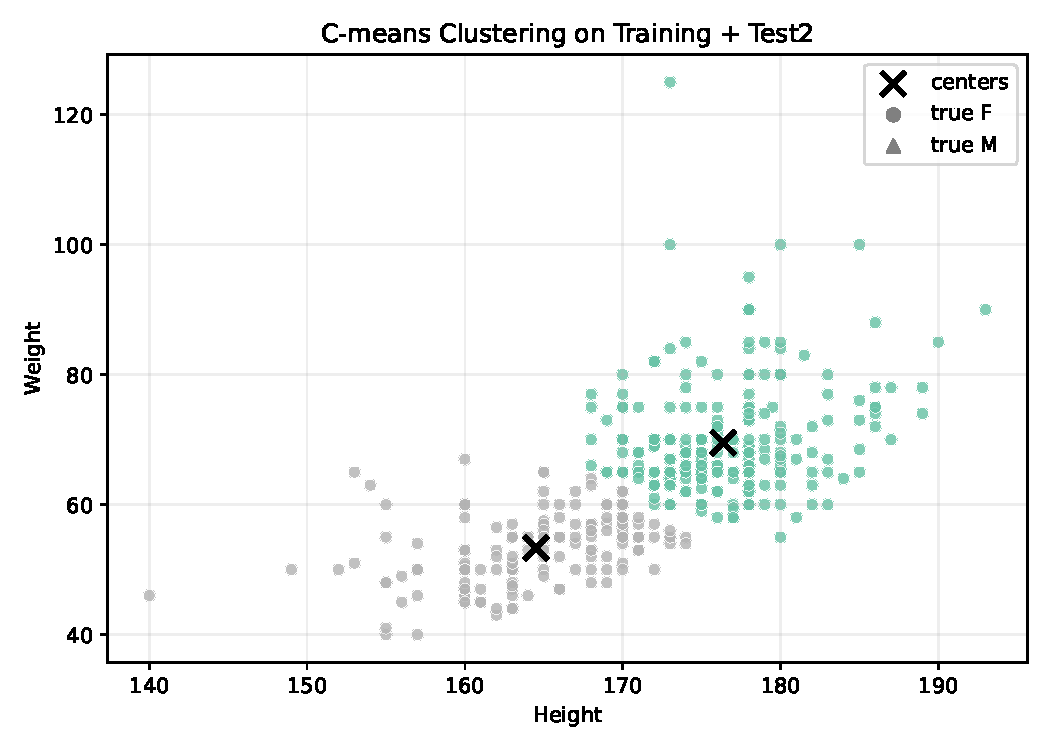
\includegraphics[width=0.74\textwidth]{figures/experiment5/cmeans_combined_2clusters.pdf}
\caption{训练集与 test2 合并后的 C 均值聚类结果，$C=2$}
\label{fig:exp5_cmeans_combined}
\end{figure}

合并数据上不同类别数的指标如图 \ref{fig:exp5_k_combined} 所示。

\begin{figure}[H]
\centering
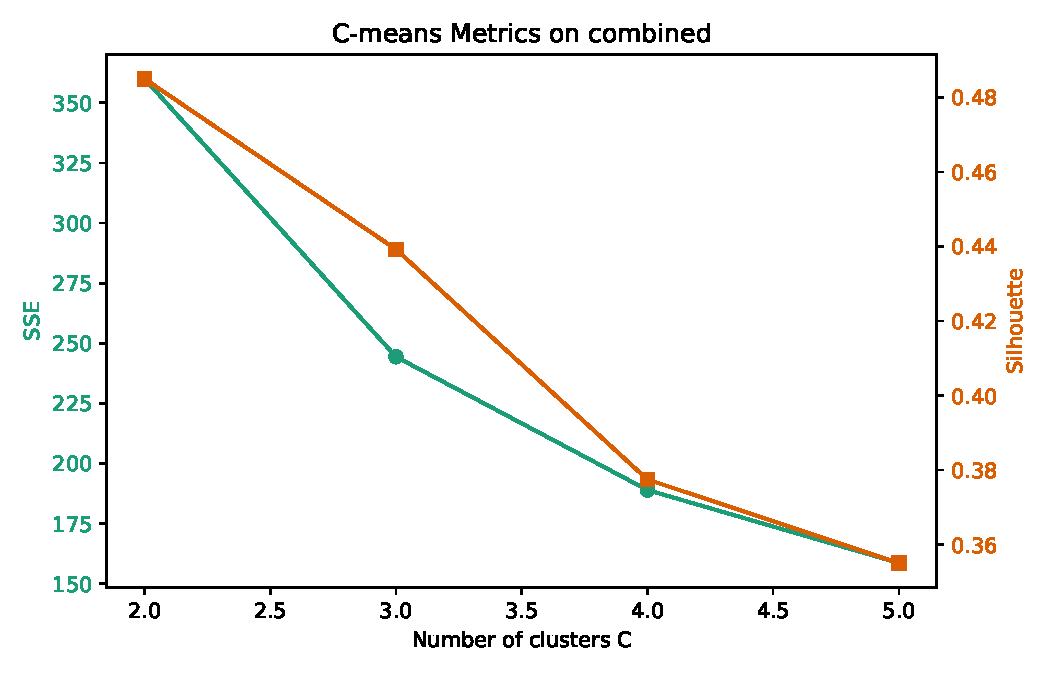
\includegraphics[width=0.74\textwidth]{figures/experiment5/cmeans_k_metrics_combined.pdf}
\caption{训练集与 test2 合并后不同类别数的 C 均值聚类指标}
\label{fig:exp5_k_combined}
\end{figure}

对合并数据使用 Ward 分级聚类并取两类，结果如图 \ref{fig:exp5_hier_combined} 所示。

\begin{figure}[H]
\centering
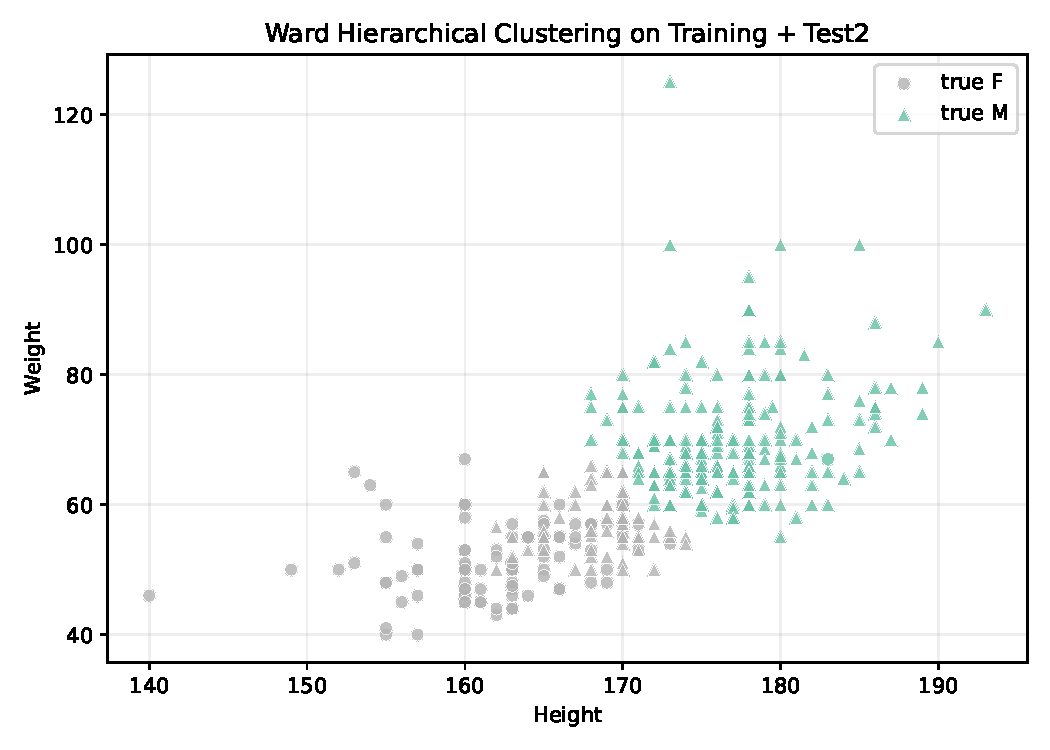
\includegraphics[width=0.74\textwidth]{figures/experiment5/hierarchical_combined_2clusters.pdf}
\caption{训练集与 test2 合并后的 Ward 分级聚类结果，$C=2$}
\label{fig:exp5_hier_combined}
\end{figure}

合并数据中 C 均值 $C=2$ 的轮廓系数为 0.4850，ARI 为 0.4693，性别匹配率为 84.50\%；Ward 分级聚类的轮廓系数为 0.4739，性别匹配率为 82.50\%。与训练集相比，合并数据的轮廓系数略有下降，说明新增样本增加了类内变化和边界重叠；但 $C=2$ 仍然具有最高轮廓系数，说明合理类别数仍可认为是 2。

\begin{table}[H]
\centering
\caption{实验五聚类结果汇总}
\label{tab:exp5_summary}
\small
\begin{tabular}{p{2.4cm}p{3.0cm}p{1.4cm}p{1.8cm}p{1.8cm}p{2.0cm}}
\toprule
数据集 & 方法 & 类数 & 轮廓系数 & ARI & 性别匹配率 \\
\midrule
训练集 & C 均值 & 2 & 0.5108 & 0.4850 & 85.00\% \\
训练集 & Ward 分级聚类 & 2 & 0.5049 & 0.3789 & 81.00\% \\
训练集+test2 & C 均值 & 2 & 0.4850 & 0.4693 & 84.50\% \\
训练集+test2 & Ward 分级聚类 & 2 & 0.4739 & 0.4172 & 82.50\% \\
\bottomrule
\end{tabular}

\end{table}

\subsection{综合实验结果与分析总结}

综合表 \ref{tab:exp5_summary} 和各图可以得到以下结论：
\begin{itemize}
  \item C 均值在训练集上取 $C=2$ 时性别匹配率为 85.00\%，说明身高体重空间中存在与性别相关的自然聚类结构。
  \item 不同初始中心会造成少量边界样本变化，但 SSE 和性别匹配率波动较小，说明该数据集上 C 均值结果较稳定。
  \item 随着类别数从 2 增加到 5，SSE 持续下降，但轮廓系数下降，说明继续增加类别数会把自然的两类结构过度切分。
  \item Ward 分级聚类不需要随机初始化，能展示层次结构，但本数据集上性别匹配率略低于 C 均值。
  \item 加入 test2 后，样本量增大且男生比例提高，聚类指标略有下降，但两类结构仍然最合理。
\end{itemize}

聚类结果与前面监督分类实验相互印证：身高和体重确实具有性别区分信息，但男女样本在边界区域存在重叠，因此无监督聚类无法完全恢复真实性别标签。聚类算法发现的是数据几何结构，而不是语义标签本身。

\subsection{体会}

通过本实验可以体会到，聚类与分类的目标不同。分类器利用标签学习判别边界，而聚类只根据距离和分布自动分组。即使聚类结果与性别标签较一致，也只能说明特征空间中存在相应结构，不能说明聚类算法真正理解了“性别”这个类别含义。

C 均值算法实现简单、效率高，适合低维连续特征；但它对类别数、初始中心和标准化处理敏感。分级聚类能够展示更丰富的层次关系，适合观察样本合并过程。实验中两种方法都支持 $C=2$ 是较合理类别数，这与男女数据集的真实类别数一致，也说明身高和体重是较有效的聚类特征。

\clearpage
\section{总体总结}

五个实验从参数 Bayes 分类、非参数估计、Fisher 线性判别、K-L 特征提取、K-L 应用和聚类分析等角度完整覆盖了模式识别课程中的重要方法。总体来看，男女身高体重数据结构清晰，适合用于理解分类边界、特征投影和聚类结构之间的关系；图像类实验则展示了 K-L/PCA 在高维数据降维中的应用价值。后续若进一步完善，可以补充更多超参数敏感性分析和更复杂数据集上的泛化比较。
\end{document}
